

%#########################1########################

 \cajita{%
Evolución de la población }%
{%
Las proyecciones de población a nivel nacional indican que para el 30 de junio de 2015 habrían 16.176 millones de personas.

Según la Encuesta Nacional de Condiciones de Vida de 2014, el 51.5\% de la población era mujer y el 38.8\% se autoidentificaba como indígena. }%
{%
 Evolución de la población} %
{%
 República de Guatemala, serie histórica, en miles} %
{%
 \begin{tikzpicture}[x=1pt,y=1pt]  % Created by tikzDevice version 0.9 on 2016-03-03 01:12:06
% !TEX encoding = UTF-8 Unicode
\definecolor{fillColor}{RGB}{255,255,255}
\path[use as bounding box,fill=fillColor,fill opacity=0.00] (0,0) rectangle (289.08,198.74);
\begin{scope}
\path[clip] (  0.00,  0.00) rectangle (289.08,198.74);

\path[] (  0.00,  0.00) rectangle (289.08,198.74);
\end{scope}
\begin{scope}
\path[clip] (  0.00,  0.00) rectangle (289.08,198.74);

\path[] ( 12.62, 15.61) rectangle (280.54,191.48);

\path[] ( 12.62, 21.50) --
	(280.54, 21.50);

\path[] ( 12.62, 63.55) --
	(280.54, 63.55);

\path[] ( 12.62,105.60) --
	(280.54,105.60);

\path[] ( 12.62,147.65) --
	(280.54,147.65);

\path[] ( 12.62,189.70) --
	(280.54,189.70);

\path[] ( 12.62, 42.52) --
	(280.54, 42.52);

\path[] ( 12.62, 84.58) --
	(280.54, 84.58);

\path[] ( 12.62,126.63) --
	(280.54,126.63);

\path[] ( 12.62,168.68) --
	(280.54,168.68);

\path[] ( 43.53, 15.61) --
	( 43.53,191.48);

\path[] ( 95.06, 15.61) --
	( 95.06,191.48);

\path[] (146.58, 15.61) --
	(146.58,191.48);

\path[] (198.11, 15.61) --
	(198.11,191.48);

\path[] (249.63, 15.61) --
	(249.63,191.48);
\definecolor{drawColor}{RGB}{0,0,255}

\path[draw=drawColor,line width= 1.7pt,line join=round] ( 43.53, 60.50) --
	( 95.06, 90.75) --
	(146.58,121.44) --
	(198.11,152.42) --
	(249.63,183.49);
\definecolor{drawColor}{RGB}{0,0,0}

\node[text=drawColor,anchor=base,inner sep=0pt, outer sep=0pt, scale=  1.02] at ( 43.53, 48.59) {14,713.8};

\node[text=drawColor,anchor=base east,inner sep=0pt, outer sep=0pt, scale=  1.02] at ( 88.80, 90.75) {15,073.4};

\node[text=drawColor,anchor=base east,inner sep=0pt, outer sep=0pt, scale=  1.02] at (140.33,121.44) {15,438.4};

\node[text=drawColor,anchor=base east,inner sep=0pt, outer sep=0pt, scale=  1.02] at (191.85,152.42) {15,806.7};

\node[text=drawColor,anchor=base,inner sep=0pt, outer sep=0pt, scale=  1.02] at (249.63,187.46) {16,176.1};

\path[draw=drawColor,line width= 0.1pt,line join=round] ( 12.62, 23.61) -- (280.54, 23.61);

\path[] ( 12.62, 15.61) rectangle (280.54,191.48);
\end{scope}
\begin{scope}
\path[clip] (  0.00,  0.00) rectangle (289.08,198.74);

\path[] ( 12.62, 15.61) --
	( 12.62,191.48);
\end{scope}
\begin{scope}
\path[clip] (  0.00,  0.00) rectangle (289.08,198.74);
\definecolor{drawColor}{RGB}{255,255,255}

\node[text=drawColor,text opacity=0.00,anchor=base east,inner sep=0pt, outer sep=0pt, scale=  1.00] at (  7.67, 38.62) {14500};

\node[text=drawColor,text opacity=0.00,anchor=base east,inner sep=0pt, outer sep=0pt, scale=  1.00] at (  7.67, 80.67) {15000};

\node[text=drawColor,text opacity=0.00,anchor=base east,inner sep=0pt, outer sep=0pt, scale=  1.00] at (  7.67,122.72) {15500};

\node[text=drawColor,text opacity=0.00,anchor=base east,inner sep=0pt, outer sep=0pt, scale=  1.00] at (  7.67,164.77) {16000};
\end{scope}
\begin{scope}
\path[clip] (  0.00,  0.00) rectangle (289.08,198.74);

\path[] (  9.87, 42.52) --
	( 12.62, 42.52);

\path[] (  9.87, 84.58) --
	( 12.62, 84.58);

\path[] (  9.87,126.63) --
	( 12.62,126.63);

\path[] (  9.87,168.68) --
	( 12.62,168.68);
\end{scope}
\begin{scope}
\path[clip] (  0.00,  0.00) rectangle (289.08,198.74);

\path[] ( 12.62, 15.61) --
	(280.54, 15.61);
\end{scope}
\begin{scope}
\path[clip] (  0.00,  0.00) rectangle (289.08,198.74);

\path[] ( 43.53, 12.86) --
	( 43.53, 15.61);

\path[] ( 95.06, 12.86) --
	( 95.06, 15.61);

\path[] (146.58, 12.86) --
	(146.58, 15.61);

\path[] (198.11, 12.86) --
	(198.11, 15.61);

\path[] (249.63, 12.86) --
	(249.63, 15.61);
\end{scope}
\begin{scope}
\path[clip] (  0.00,  0.00) rectangle (289.08,198.74);
\definecolor{drawColor}{RGB}{0,0,0}

\node[text=drawColor,anchor=base,inner sep=0pt, outer sep=0pt, scale=  1.00] at ( 43.53,  2.85) {2011};

\node[text=drawColor,anchor=base,inner sep=0pt, outer sep=0pt, scale=  1.00] at ( 95.06,  2.85) {2012};

\node[text=drawColor,anchor=base,inner sep=0pt, outer sep=0pt, scale=  1.00] at (146.58,  2.85) {2013};

\node[text=drawColor,anchor=base,inner sep=0pt, outer sep=0pt, scale=  1.00] at (198.11,  2.85) {2014};

\node[text=drawColor,anchor=base,inner sep=0pt, outer sep=0pt, scale=  1.00] at (249.63,  2.85) {2015};
\end{scope}
  \end{tikzpicture}}%
{%
 Instituto Nacional de Estadística} %



%#################################2#######################


 \cajita{%
 	Densidad de población }%
 {%
La densidad población en el 2015 fue de 149 habitantes por kilómetro cuadrado.

 \textollamada[*]{A la densidad calculada como el número promedio de habitantes del departamento, también se le denomina densidad relativa. Este, al ser un promedio, no muestra las diferencias dentro del territorio analizado.}
\textollamada[*]{De acuerdo a la definición del banco mundial, este indicador relaciona la cantidad de residentes sin importar su estado legal o de ciudadanía y el área de tierra superficial total de un país, sin incluir la superficie cubierta por masas de agua interiores.}}%
 {%
 Evolución en la densidad de la población} %
 {%
 	República de Guatemala, serie histórica, habitantes por kilómetro cuadrado} %
 {%
 	\begin{tikzpicture}[x=1pt,y=1pt]  % Created by tikzDevice version 0.9 on 2016-03-03 01:12:07
% !TEX encoding = UTF-8 Unicode
\definecolor{fillColor}{RGB}{255,255,255}
\path[use as bounding box,fill=fillColor,fill opacity=0.00] (0,0) rectangle (289.08,198.74);
\begin{scope}
\path[clip] (  0.00,  0.00) rectangle (289.08,198.74);

\path[] (  0.00,  0.00) rectangle (289.08,198.74);
\end{scope}
\begin{scope}
\path[clip] (  0.00,  0.00) rectangle (289.08,198.74);

\path[] (  3.86, 15.61) rectangle (280.54,191.48);

\path[] (  3.86, 36.45) --
	(280.54, 36.45);

\path[] (  3.86, 82.24) --
	(280.54, 82.24);

\path[] (  3.86,128.03) --
	(280.54,128.03);

\path[] (  3.86,173.82) --
	(280.54,173.82);

\path[] (  3.86, 59.35) --
	(280.54, 59.35);

\path[] (  3.86,105.13) --
	(280.54,105.13);

\path[] (  3.86,150.92) --
	(280.54,150.92);

\path[] ( 35.79, 15.61) --
	( 35.79,191.48);

\path[] ( 88.99, 15.61) --
	( 88.99,191.48);

\path[] (142.20, 15.61) --
	(142.20,191.48);

\path[] (195.41, 15.61) --
	(195.41,191.48);

\path[] (248.62, 15.61) --
	(248.62,191.48);
\definecolor{drawColor}{RGB}{0,0,255}

\path[draw=drawColor,line width= 1.7pt,line join=round] ( 35.79, 60.50) --
	( 88.99, 90.75) --
	(142.20,121.44) --
	(195.41,152.42) --
	(248.62,183.49);
\definecolor{drawColor}{RGB}{0,0,0}

\node[text=drawColor,anchor=base,inner sep=0pt, outer sep=0pt, scale=  1.02] at ( 35.79, 48.59) {135.1};

\node[text=drawColor,anchor=base east,inner sep=0pt, outer sep=0pt, scale=  1.02] at ( 84.98, 90.75) {138.4};

\node[text=drawColor,anchor=base east,inner sep=0pt, outer sep=0pt, scale=  1.02] at (138.18,121.44) {141.8};

\node[text=drawColor,anchor=base east,inner sep=0pt, outer sep=0pt, scale=  1.02] at (191.39,152.42) {145.2};

\node[text=drawColor,anchor=base,inner sep=0pt, outer sep=0pt, scale=  1.02] at (248.62,187.46) {148.6};

\path[draw=drawColor,line width= 0.1pt,line join=round] (  3.86, 23.61) -- (280.54, 23.61);

\path[] (  3.86, 15.61) rectangle (280.54,191.48);
\end{scope}
\begin{scope}
\path[clip] (  0.00,  0.00) rectangle (289.08,198.74);

\path[] (  3.86, 15.61) --
	(  3.86,191.48);
\end{scope}
\begin{scope}
\path[clip] (  0.00,  0.00) rectangle (289.08,198.74);

\path[] (  1.11, 59.35) --
	(  3.86, 59.35);

\path[] (  1.11,105.13) --
	(  3.86,105.13);

\path[] (  1.11,150.92) --
	(  3.86,150.92);
\end{scope}
\begin{scope}
\path[clip] (  0.00,  0.00) rectangle (289.08,198.74);

\path[] (  3.86, 15.61) --
	(280.54, 15.61);
\end{scope}
\begin{scope}
\path[clip] (  0.00,  0.00) rectangle (289.08,198.74);

\path[] ( 35.79, 12.86) --
	( 35.79, 15.61);

\path[] ( 88.99, 12.86) --
	( 88.99, 15.61);

\path[] (142.20, 12.86) --
	(142.20, 15.61);

\path[] (195.41, 12.86) --
	(195.41, 15.61);

\path[] (248.62, 12.86) --
	(248.62, 15.61);
\end{scope}
\begin{scope}
\path[clip] (  0.00,  0.00) rectangle (289.08,198.74);
\definecolor{drawColor}{RGB}{0,0,0}

\node[text=drawColor,anchor=base,inner sep=0pt, outer sep=0pt, scale=  1.00] at ( 35.79,  2.85) {2011};

\node[text=drawColor,anchor=base,inner sep=0pt, outer sep=0pt, scale=  1.00] at ( 88.99,  2.85) {2012};

\node[text=drawColor,anchor=base,inner sep=0pt, outer sep=0pt, scale=  1.00] at (142.20,  2.85) {2013};

\node[text=drawColor,anchor=base,inner sep=0pt, outer sep=0pt, scale=  1.00] at (195.41,  2.85) {2014};

\node[text=drawColor,anchor=base,inner sep=0pt, outer sep=0pt, scale=  1.00] at (248.62,  2.85) {2015};
\end{scope}
  \end{tikzpicture}}%
 {%
 	Instituto Nacional de Estadística} %
 
 
 
 
 
%%%%%%%%%%%%%%%%%%%%%%%%%%%%%%%%%%3%%%%%%%%%%%%%%%%%%%%%%%%

 \cajita{%
 	Población por grupos de edad, año 2008 }%
 {%
 Se muestra la distribución de la población en el 2008 según grupos quinquenales de edad. En ella se destaca que la población entre 0 y 4 años era la más representativa. El 52.3\% era menor de 20 años.
   }%
 {%
 	Distribución de la población por grupos quinquenales de edad} %
 {%
 	República de Guatemala, año 2008, en porcentaje} %
 {%
 	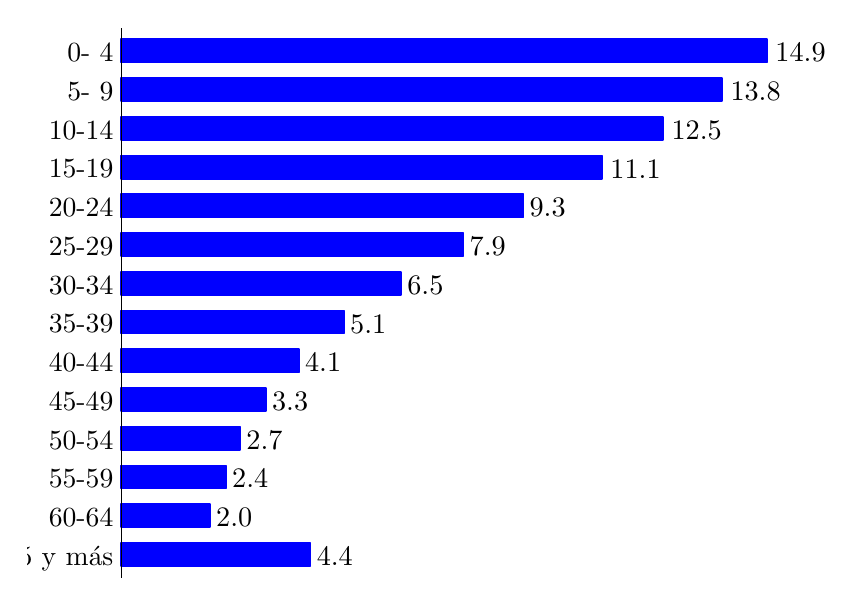
\begin{tikzpicture}[x=1pt,y=1pt]  % Created by tikzDevice version 0.9 on 2016-03-03 01:20:43
% !TEX encoding = UTF-8 Unicode
\definecolor{fillColor}{RGB}{255,255,255}
\path[use as bounding box,fill=fillColor,fill opacity=0.00] (0,0) rectangle (289.08,198.74);
\begin{scope}
\path[clip] (  0.00,  0.00) rectangle (289.08,198.74);

\path[] (  0.00,  0.00) rectangle (289.08,198.74);
\end{scope}
\begin{scope}
\path[clip] (  0.00,  0.00) rectangle (289.08,198.74);

\path[] ( 33.72,  0.00) rectangle (267.09,198.74);

\path[] ( 33.72,  8.40) --
	(267.09,  8.40);

\path[] ( 33.72, 22.39) --
	(267.09, 22.39);

\path[] ( 33.72, 36.39) --
	(267.09, 36.39);

\path[] ( 33.72, 50.39) --
	(267.09, 50.39);

\path[] ( 33.72, 64.38) --
	(267.09, 64.38);

\path[] ( 33.72, 78.38) --
	(267.09, 78.38);

\path[] ( 33.72, 92.37) --
	(267.09, 92.37);

\path[] ( 33.72,106.37) --
	(267.09,106.37);

\path[] ( 33.72,120.37) --
	(267.09,120.37);

\path[] ( 33.72,134.36) --
	(267.09,134.36);

\path[] ( 33.72,148.36) --
	(267.09,148.36);

\path[] ( 33.72,162.35) --
	(267.09,162.35);

\path[] ( 33.72,176.35) --
	(267.09,176.35);

\path[] ( 33.72,190.34) --
	(267.09,190.34);
\definecolor{drawColor}{RGB}{0,0,255}
\definecolor{fillColor}{RGB}{0,0,255}

\path[draw=drawColor,line width= 0.6pt,line join=round,fill=fillColor] ( 33.72,  4.20) rectangle (102.23, 12.60);

\path[draw=drawColor,line width= 0.6pt,line join=round,fill=fillColor] ( 33.72, 18.19) rectangle ( 65.88, 26.59);

\path[draw=drawColor,line width= 0.6pt,line join=round,fill=fillColor] ( 33.72, 32.19) rectangle ( 71.66, 40.59);

\path[draw=drawColor,line width= 0.6pt,line join=round,fill=fillColor] ( 33.72, 46.19) rectangle ( 76.82, 54.58);

\path[draw=drawColor,line width= 0.6pt,line join=round,fill=fillColor] ( 33.72, 60.18) rectangle ( 86.10, 68.58);

\path[draw=drawColor,line width= 0.6pt,line join=round,fill=fillColor] ( 33.72, 74.18) rectangle ( 98.00, 82.58);

\path[draw=drawColor,line width= 0.6pt,line join=round,fill=fillColor] ( 33.72, 88.17) rectangle (114.32, 96.57);

\path[draw=drawColor,line width= 0.6pt,line join=round,fill=fillColor] ( 33.72,102.17) rectangle (134.96,110.57);

\path[draw=drawColor,line width= 0.6pt,line join=round,fill=fillColor] ( 33.72,116.17) rectangle (157.49,124.56);

\path[draw=drawColor,line width= 0.6pt,line join=round,fill=fillColor] ( 33.72,130.16) rectangle (179.13,138.56);

\path[draw=drawColor,line width= 0.6pt,line join=round,fill=fillColor] ( 33.72,144.16) rectangle (207.45,152.56);

\path[draw=drawColor,line width= 0.6pt,line join=round,fill=fillColor] ( 33.72,158.15) rectangle (229.56,166.55);

\path[draw=drawColor,line width= 0.6pt,line join=round,fill=fillColor] ( 33.72,172.15) rectangle (250.84,180.55);

\path[draw=drawColor,line width= 0.6pt,line join=round,fill=fillColor] ( 33.72,186.15) rectangle (267.09,194.54);
\definecolor{drawColor}{RGB}{0,0,0}

\path[draw=drawColor,line width= 0.1pt,line join=round] ( 33.72,  0.00) -- ( 33.72,198.74);

\node[text=drawColor,anchor=base west,inner sep=0pt, outer sep=0pt, scale=  1.02] at (104.47,  4.43) {4.4};

\node[text=drawColor,anchor=base west,inner sep=0pt, outer sep=0pt, scale=  1.02] at ( 68.12, 18.42) {2.0};

\node[text=drawColor,anchor=base west,inner sep=0pt, outer sep=0pt, scale=  1.02] at ( 73.90, 32.42) {2.4};

\node[text=drawColor,anchor=base west,inner sep=0pt, outer sep=0pt, scale=  1.02] at ( 79.05, 46.41) {2.7};

\node[text=drawColor,anchor=base west,inner sep=0pt, outer sep=0pt, scale=  1.02] at ( 88.33, 60.41) {3.3};

\node[text=drawColor,anchor=base west,inner sep=0pt, outer sep=0pt, scale=  1.02] at (100.23, 74.41) {4.1};

\node[text=drawColor,anchor=base west,inner sep=0pt, outer sep=0pt, scale=  1.02] at (116.56, 88.40) {5.1};

\node[text=drawColor,anchor=base west,inner sep=0pt, outer sep=0pt, scale=  1.02] at (137.19,102.40) {6.5};

\node[text=drawColor,anchor=base west,inner sep=0pt, outer sep=0pt, scale=  1.02] at (159.73,116.39) {7.9};

\node[text=drawColor,anchor=base west,inner sep=0pt, outer sep=0pt, scale=  1.02] at (181.37,130.39) {9.3};

\node[text=drawColor,anchor=base west,inner sep=0pt, outer sep=0pt, scale=  1.02] at (210.58,144.39) {11.1};

\node[text=drawColor,anchor=base west,inner sep=0pt, outer sep=0pt, scale=  1.02] at (232.69,158.38) {12.5};

\node[text=drawColor,anchor=base west,inner sep=0pt, outer sep=0pt, scale=  1.02] at (253.97,172.38) {13.8};

\node[text=drawColor,anchor=base west,inner sep=0pt, outer sep=0pt, scale=  1.02] at (270.21,186.37) {14.9};

\path[] ( 33.72,  0.00) rectangle (267.09,198.74);
\end{scope}
\begin{scope}
\path[clip] (  0.00,  0.00) rectangle (289.08,198.74);

\path[] ( 33.72,  0.00) --
	( 33.72,198.74);
\end{scope}
\begin{scope}
\path[clip] (  0.00,  0.00) rectangle (289.08,198.74);
\definecolor{drawColor}{RGB}{0,0,0}

\node[text=drawColor,anchor=base east,inner sep=0pt, outer sep=0pt, scale=  1.00] at ( 30.97,  4.49) {65 y más};

\node[text=drawColor,anchor=base east,inner sep=0pt, outer sep=0pt, scale=  1.00] at ( 30.97, 18.49) {60-64};

\node[text=drawColor,anchor=base east,inner sep=0pt, outer sep=0pt, scale=  1.00] at ( 30.97, 32.48) {55-59};

\node[text=drawColor,anchor=base east,inner sep=0pt, outer sep=0pt, scale=  1.00] at ( 30.97, 46.48) {50-54};

\node[text=drawColor,anchor=base east,inner sep=0pt, outer sep=0pt, scale=  1.00] at ( 30.97, 60.47) {45-49};

\node[text=drawColor,anchor=base east,inner sep=0pt, outer sep=0pt, scale=  1.00] at ( 30.97, 74.47) {40-44};

\node[text=drawColor,anchor=base east,inner sep=0pt, outer sep=0pt, scale=  1.00] at ( 30.97, 88.46) {35-39};

\node[text=drawColor,anchor=base east,inner sep=0pt, outer sep=0pt, scale=  1.00] at ( 30.97,102.46) {30-34};

\node[text=drawColor,anchor=base east,inner sep=0pt, outer sep=0pt, scale=  1.00] at ( 30.97,116.46) {25-29};

\node[text=drawColor,anchor=base east,inner sep=0pt, outer sep=0pt, scale=  1.00] at ( 30.97,130.45) {20-24};

\node[text=drawColor,anchor=base east,inner sep=0pt, outer sep=0pt, scale=  1.00] at ( 30.97,144.45) {15-19};

\node[text=drawColor,anchor=base east,inner sep=0pt, outer sep=0pt, scale=  1.00] at ( 30.97,158.44) {10-14};

\node[text=drawColor,anchor=base east,inner sep=0pt, outer sep=0pt, scale=  1.00] at ( 30.97,172.44) {5- 9};

\node[text=drawColor,anchor=base east,inner sep=0pt, outer sep=0pt, scale=  1.00] at ( 30.97,186.44) {0- 4};
\end{scope}
\begin{scope}
\path[clip] (  0.00,  0.00) rectangle (289.08,198.74);

\path[] ( 30.97,  8.40) --
	( 33.72,  8.40);

\path[] ( 30.97, 22.39) --
	( 33.72, 22.39);

\path[] ( 30.97, 36.39) --
	( 33.72, 36.39);

\path[] ( 30.97, 50.39) --
	( 33.72, 50.39);

\path[] ( 30.97, 64.38) --
	( 33.72, 64.38);

\path[] ( 30.97, 78.38) --
	( 33.72, 78.38);

\path[] ( 30.97, 92.37) --
	( 33.72, 92.37);

\path[] ( 30.97,106.37) --
	( 33.72,106.37);

\path[] ( 30.97,120.37) --
	( 33.72,120.37);

\path[] ( 30.97,134.36) --
	( 33.72,134.36);

\path[] ( 30.97,148.36) --
	( 33.72,148.36);

\path[] ( 30.97,162.35) --
	( 33.72,162.35);

\path[] ( 30.97,176.35) --
	( 33.72,176.35);

\path[] ( 30.97,190.34) --
	( 33.72,190.34);
\end{scope}
  \end{tikzpicture}}%
 {%
 	Instituto Nacional de Estadística} %
 
 %%%%%%%%%%%%%%%%%%%%%%%%%%%%%%%%%%4%%%%%%%%%%%%%%%%%%%%%%%%
 
 \cajita{%
 	Población por grupos de edad, año 2015 }%
 {%
En la distribución porcentual de la población del 2015 por grupos de edad se muestra que la población joven menor de 20 años representó el 50.5\%, ligeramente menor a lo observado en el 2008. 

En general, la distribución según edad en los últimos 7 años cambió ligeramente, reduciéndose la población joven. }%
 {%
 	Distribución de la población por grupos quinquenales de edad} %
 {%
 	República de Guatemala, año 2015, en porcentaje} %
 {%
 	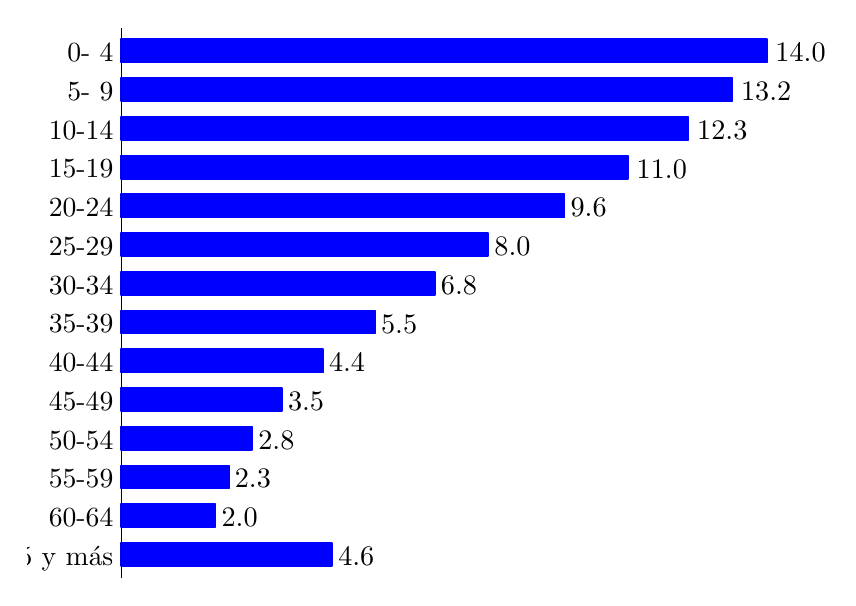
\begin{tikzpicture}[x=1pt,y=1pt]  % Created by tikzDevice version 0.9 on 2016-03-03 01:22:03
% !TEX encoding = UTF-8 Unicode
\definecolor{fillColor}{RGB}{255,255,255}
\path[use as bounding box,fill=fillColor,fill opacity=0.00] (0,0) rectangle (289.08,198.74);
\begin{scope}
\path[clip] (  0.00,  0.00) rectangle (289.08,198.74);

\path[] (  0.00,  0.00) rectangle (289.08,198.74);
\end{scope}
\begin{scope}
\path[clip] (  0.00,  0.00) rectangle (289.08,198.74);

\path[] ( 33.72,  0.00) rectangle (267.09,198.74);

\path[] ( 33.72,  8.40) --
	(267.09,  8.40);

\path[] ( 33.72, 22.39) --
	(267.09, 22.39);

\path[] ( 33.72, 36.39) --
	(267.09, 36.39);

\path[] ( 33.72, 50.39) --
	(267.09, 50.39);

\path[] ( 33.72, 64.38) --
	(267.09, 64.38);

\path[] ( 33.72, 78.38) --
	(267.09, 78.38);

\path[] ( 33.72, 92.37) --
	(267.09, 92.37);

\path[] ( 33.72,106.37) --
	(267.09,106.37);

\path[] ( 33.72,120.37) --
	(267.09,120.37);

\path[] ( 33.72,134.36) --
	(267.09,134.36);

\path[] ( 33.72,148.36) --
	(267.09,148.36);

\path[] ( 33.72,162.35) --
	(267.09,162.35);

\path[] ( 33.72,176.35) --
	(267.09,176.35);

\path[] ( 33.72,190.34) --
	(267.09,190.34);
\definecolor{drawColor}{RGB}{0,0,255}
\definecolor{fillColor}{RGB}{0,0,255}

\path[draw=drawColor,line width= 0.6pt,line join=round,fill=fillColor] ( 33.72,  4.20) rectangle (110.00, 12.60);

\path[draw=drawColor,line width= 0.6pt,line join=round,fill=fillColor] ( 33.72, 18.19) rectangle ( 67.84, 26.59);

\path[draw=drawColor,line width= 0.6pt,line join=round,fill=fillColor] ( 33.72, 32.19) rectangle ( 72.63, 40.59);

\path[draw=drawColor,line width= 0.6pt,line join=round,fill=fillColor] ( 33.72, 46.19) rectangle ( 81.11, 54.58);

\path[draw=drawColor,line width= 0.6pt,line join=round,fill=fillColor] ( 33.72, 60.18) rectangle ( 91.84, 68.58);

\path[draw=drawColor,line width= 0.6pt,line join=round,fill=fillColor] ( 33.72, 74.18) rectangle (106.66, 82.58);

\path[draw=drawColor,line width= 0.6pt,line join=round,fill=fillColor] ( 33.72, 88.17) rectangle (125.49, 96.57);

\path[draw=drawColor,line width= 0.6pt,line join=round,fill=fillColor] ( 33.72,102.17) rectangle (147.08,110.57);

\path[draw=drawColor,line width= 0.6pt,line join=round,fill=fillColor] ( 33.72,116.17) rectangle (166.43,124.56);

\path[draw=drawColor,line width= 0.6pt,line join=round,fill=fillColor] ( 33.72,130.16) rectangle (193.95,138.56);

\path[draw=drawColor,line width= 0.6pt,line join=round,fill=fillColor] ( 33.72,144.16) rectangle (216.94,152.56);

\path[draw=drawColor,line width= 0.6pt,line join=round,fill=fillColor] ( 33.72,158.15) rectangle (238.83,166.55);

\path[draw=drawColor,line width= 0.6pt,line join=round,fill=fillColor] ( 33.72,172.15) rectangle (254.69,180.55);

\path[draw=drawColor,line width= 0.6pt,line join=round,fill=fillColor] ( 33.72,186.15) rectangle (267.09,194.54);
\definecolor{drawColor}{RGB}{0,0,0}

\path[draw=drawColor,line width= 0.1pt,line join=round] ( 33.72,  0.00) -- ( 33.72,198.74);

\node[text=drawColor,anchor=base west,inner sep=0pt, outer sep=0pt, scale=  1.02] at (112.24,  4.43) {4.6};

\node[text=drawColor,anchor=base west,inner sep=0pt, outer sep=0pt, scale=  1.02] at ( 70.08, 18.42) {2.0};

\node[text=drawColor,anchor=base west,inner sep=0pt, outer sep=0pt, scale=  1.02] at ( 74.87, 32.42) {2.3};

\node[text=drawColor,anchor=base west,inner sep=0pt, outer sep=0pt, scale=  1.02] at ( 83.35, 46.41) {2.8};

\node[text=drawColor,anchor=base west,inner sep=0pt, outer sep=0pt, scale=  1.02] at ( 94.08, 60.41) {3.5};

\node[text=drawColor,anchor=base west,inner sep=0pt, outer sep=0pt, scale=  1.02] at (108.90, 74.41) {4.4};

\node[text=drawColor,anchor=base west,inner sep=0pt, outer sep=0pt, scale=  1.02] at (127.72, 88.40) {5.5};

\node[text=drawColor,anchor=base west,inner sep=0pt, outer sep=0pt, scale=  1.02] at (149.32,102.40) {6.8};

\node[text=drawColor,anchor=base west,inner sep=0pt, outer sep=0pt, scale=  1.02] at (168.67,116.39) {8.0};

\node[text=drawColor,anchor=base west,inner sep=0pt, outer sep=0pt, scale=  1.02] at (196.19,130.39) {9.6};

\node[text=drawColor,anchor=base west,inner sep=0pt, outer sep=0pt, scale=  1.02] at (220.07,144.39) {11.0};

\node[text=drawColor,anchor=base west,inner sep=0pt, outer sep=0pt, scale=  1.02] at (241.95,158.38) {12.3};

\node[text=drawColor,anchor=base west,inner sep=0pt, outer sep=0pt, scale=  1.02] at (257.81,172.38) {13.2};

\node[text=drawColor,anchor=base west,inner sep=0pt, outer sep=0pt, scale=  1.02] at (270.21,186.37) {14.0};

\path[] ( 33.72,  0.00) rectangle (267.09,198.74);
\end{scope}
\begin{scope}
\path[clip] (  0.00,  0.00) rectangle (289.08,198.74);

\path[] ( 33.72,  0.00) --
	( 33.72,198.74);
\end{scope}
\begin{scope}
\path[clip] (  0.00,  0.00) rectangle (289.08,198.74);
\definecolor{drawColor}{RGB}{0,0,0}

\node[text=drawColor,anchor=base east,inner sep=0pt, outer sep=0pt, scale=  1.00] at ( 30.97,  4.49) {65 y más};

\node[text=drawColor,anchor=base east,inner sep=0pt, outer sep=0pt, scale=  1.00] at ( 30.97, 18.49) {60-64};

\node[text=drawColor,anchor=base east,inner sep=0pt, outer sep=0pt, scale=  1.00] at ( 30.97, 32.48) {55-59};

\node[text=drawColor,anchor=base east,inner sep=0pt, outer sep=0pt, scale=  1.00] at ( 30.97, 46.48) {50-54};

\node[text=drawColor,anchor=base east,inner sep=0pt, outer sep=0pt, scale=  1.00] at ( 30.97, 60.47) {45-49};

\node[text=drawColor,anchor=base east,inner sep=0pt, outer sep=0pt, scale=  1.00] at ( 30.97, 74.47) {40-44};

\node[text=drawColor,anchor=base east,inner sep=0pt, outer sep=0pt, scale=  1.00] at ( 30.97, 88.46) {35-39};

\node[text=drawColor,anchor=base east,inner sep=0pt, outer sep=0pt, scale=  1.00] at ( 30.97,102.46) {30-34};

\node[text=drawColor,anchor=base east,inner sep=0pt, outer sep=0pt, scale=  1.00] at ( 30.97,116.46) {25-29};

\node[text=drawColor,anchor=base east,inner sep=0pt, outer sep=0pt, scale=  1.00] at ( 30.97,130.45) {20-24};

\node[text=drawColor,anchor=base east,inner sep=0pt, outer sep=0pt, scale=  1.00] at ( 30.97,144.45) {15-19};

\node[text=drawColor,anchor=base east,inner sep=0pt, outer sep=0pt, scale=  1.00] at ( 30.97,158.44) {10-14};

\node[text=drawColor,anchor=base east,inner sep=0pt, outer sep=0pt, scale=  1.00] at ( 30.97,172.44) {5- 9};

\node[text=drawColor,anchor=base east,inner sep=0pt, outer sep=0pt, scale=  1.00] at ( 30.97,186.44) {0- 4};
\end{scope}
\begin{scope}
\path[clip] (  0.00,  0.00) rectangle (289.08,198.74);

\path[] ( 30.97,  8.40) --
	( 33.72,  8.40);

\path[] ( 30.97, 22.39) --
	( 33.72, 22.39);

\path[] ( 30.97, 36.39) --
	( 33.72, 36.39);

\path[] ( 30.97, 50.39) --
	( 33.72, 50.39);

\path[] ( 30.97, 64.38) --
	( 33.72, 64.38);

\path[] ( 30.97, 78.38) --
	( 33.72, 78.38);

\path[] ( 30.97, 92.37) --
	( 33.72, 92.37);

\path[] ( 30.97,106.37) --
	( 33.72,106.37);

\path[] ( 30.97,120.37) --
	( 33.72,120.37);

\path[] ( 30.97,134.36) --
	( 33.72,134.36);

\path[] ( 30.97,148.36) --
	( 33.72,148.36);

\path[] ( 30.97,162.35) --
	( 33.72,162.35);

\path[] ( 30.97,176.35) --
	( 33.72,176.35);

\path[] ( 30.97,190.34) --
	( 33.72,190.34);
\end{scope}
  \end{tikzpicture}}%
 {%
 	Instituto Nacional de Estadística} %
 
 
 
  %%%%%%%%%%%%%%%%%%%%%%%%%%%%%%%%%%5%%%%%%%%%%%%%%%%%%%%%%%%
  
  \cajota{%
  	Población departamental del 2008 }%
  {%
 Los departamentos con el mayor número de habitantes en el 2008 fueron Guatemala, Quetzaltenango, San Marcos, Huehuetenango, Quiché y Alta Verapaz.
 
 Los departamentos que tuvieron la menor cantidad de habitantes fueron Retalhuleu, Suchitepéquez, Jalapa, Zacapa, Baja Verapaz y El Progreso. }%
  {%
  Población
  	} %
  {%
  Por departamento, año 2008, en número de habitantes} %
  {%
  	 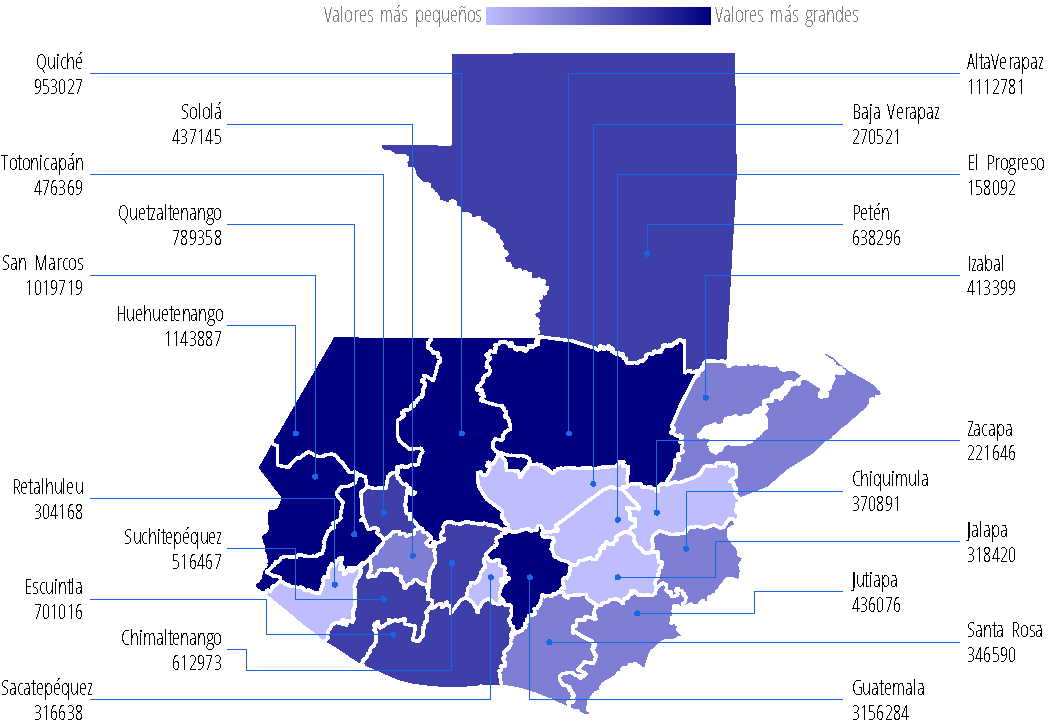
\includegraphics[width=52\cuadri]{graficas/1_02.pdf}}%
  {%
  	Instituto Nacional de Estadística} %
  
  
   %%%%%%%%%%%%%%%%%%%%%%%%%%%%%%%%%%6%%%%%%%%%%%%%%%%%%%%%%%%
   
   
    \cajota{%
    	Población departamental del 2015 }%
    {%
Al igual que en el 2008, los departamentos con la mayor cantidad de habitantes en el 2015 fueron Guatemala (el cual aumentó 6.26\% respecto al 2008), Quetzaltenango (aumentó 9.41\%), San Marcos (aumentó 10.0\%), Huehuetenango (aumentó 10.5\%), Quiché (aumentó 14.3\%) y Alta Verapaz (aumentó un 12.9\%).  }%
    {%
    Población
    } %
    {%
  Por departamento, año 2015, en número de habitantes} %
    {%
    	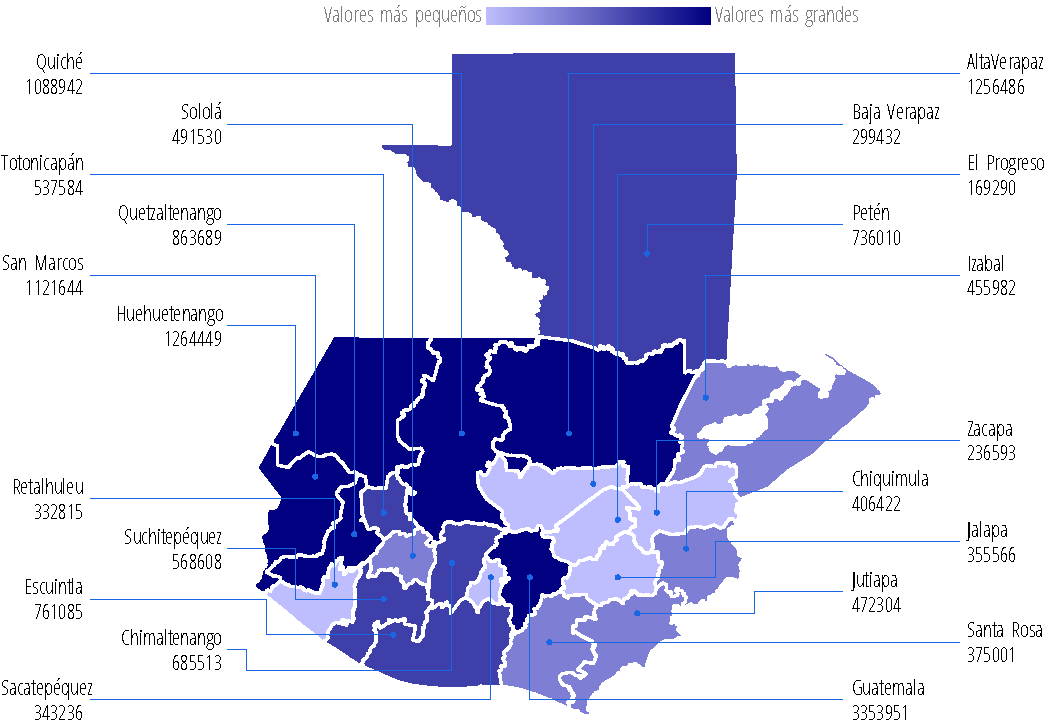
\includegraphics[width=52\cuadri]{graficas/1_03.pdf}}%
    {%
    	Instituto Nacional de Estadística} %
    
    
    %%%%%%%%%%%%%%%%%%%%%%%%%%%%%%%%%%8%%%%%%%%%%%%%%%%%%%%%%%%
    
   \cajota{%
   	Densidad poblacional departamental del 2008 }%
   {%
La densidad poblacional de la República de Guatemala en el 2008 era de 126 habitantes por kilómetro Guatemala. La misma presentó diferencias en los departamentos, donde el que tenía mayor densidad fue Guatemala con 1,408 hab/km\textsuperscript2, seguido de Sacatepéquez era de 638 hab/km\textsuperscript2, Totonicapán con 409 hab/km\textsuperscript2.

Los departamentos con menor densidad fueron Zacapa y El Progreso con 79 hab/km\textsuperscript2, Izabal con 42 hab/km\textsuperscript2 y Petén con 16 hab/km\textsuperscript2.}%
   {%
   	Densidad de la población
   } %
   {%
   	Por departamento, año 2008, hab/km\textsuperscript2} %
   {%
   	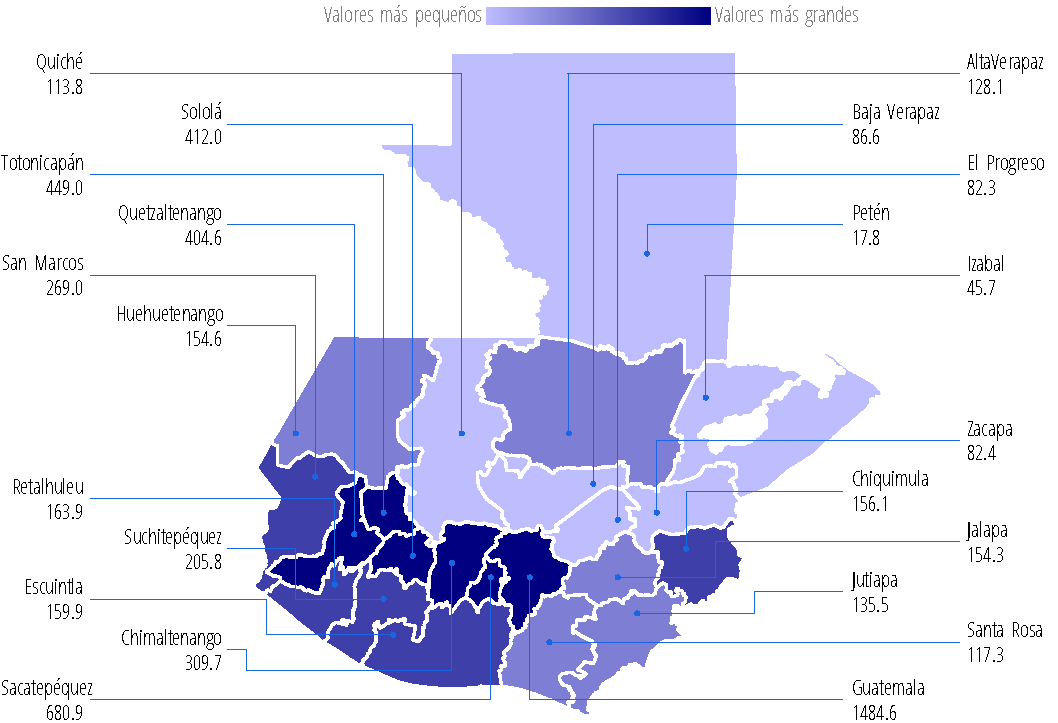
\includegraphics[width=52\cuadri]{graficas/1_05.pdf}}%
   {%
   	Instituto Nacional de Estadística} %
   
   
     %%%%%%%%%%%%%%%%%%%%%%%%%%%%%%%%%%7%%%%%%%%%%%%%%%%%%%%%%%%
     
    
     \cajota{%
     	Densidad poblacional departamental del 2015 }%
     {%
    A nivel República, la densidad poblacional para el 2015 fue de 149 hab/km\textsuperscript2.
    
    Esta presentó diferencias a nivel departamental, donde Guatemala, Sacatepéquez y Totonicapán (1,578 hab/km\textsuperscript2, 738 hab/km\textsuperscript2, 507 hab/km\textsuperscript2, respectivamente), fueron los mas densos. Estos departamentos también fueron los más densos en el 2008, y el crecimiento de los mismos fue de 12.0\%, 15.6\% y 23.9\%, respectivamente.
    
    Los departamentos menos densos fueron, al igual que en el 2008, El Progreso (88 hab/km\textsuperscript2), Zacapa (88 hab/km\textsuperscript2), Izabal (50 hab/km\textsuperscript2) y Petén (21 hab/km\textsuperscript2).
%   La densidad poblacional de la República de Guatemala en el 2008 era de 126 habitantes por kilómetro Guatemala. La misma presentó diferencias en los departamentos, donde el que tenía mayor densidad fue Guatemala con 1,408 hab/km\textsuperscript2, seguido de Sacatepéquez era de 638 hab/km\textsuperscript2, Totonicapán con 409 hab/km\textsuperscript2.
%   
%   Los departamentos con menor densidad fueron Zacapa y El Progreso con 79 hab/km\textsuperscript2, Izabal con 42 hab/km\textsuperscript2 y Petén con 16 hab/km\textsuperscript2. 
 }%
     {%
     	Densidad poblacional
     } %
     {%
      Por departamento, año 2015, hab/km\textsuperscript2} %
     {%
     	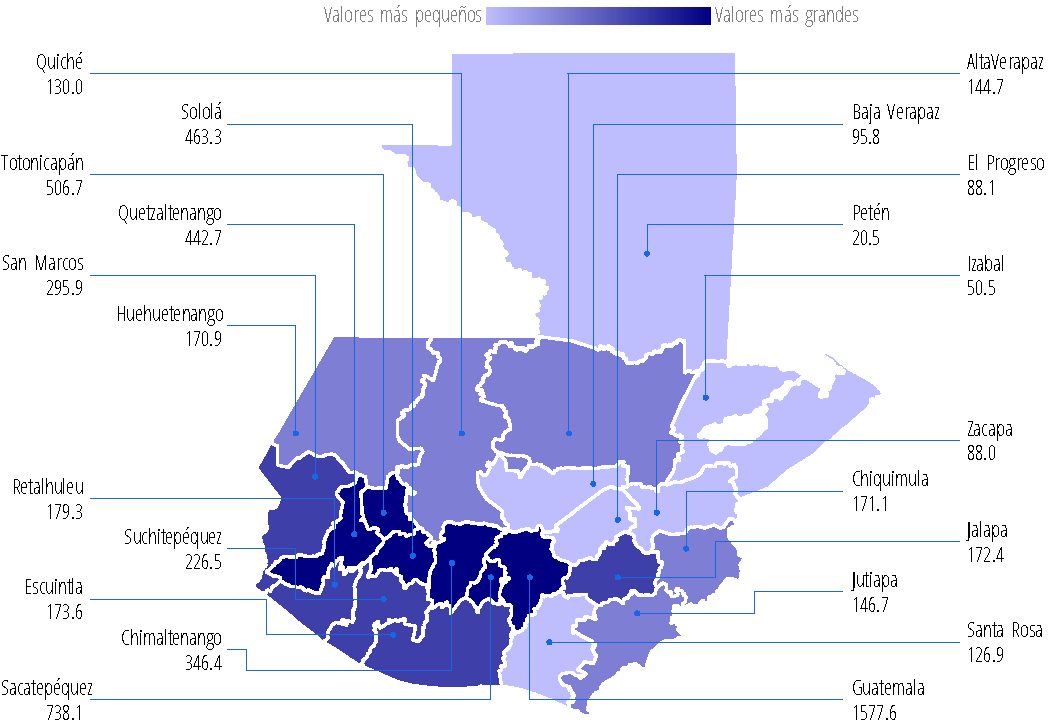
\includegraphics[width=52\cuadri]{graficas/1_06.pdf}}%
     {%
     	Instituto Nacional de Estadística} %

 %%%%%%%%%%%%%%%%%%%%%%%%%%%%%%%%%%9%%%%%%%%%%%%%%%%%%%%%%%%
 
 \cajita{%
 	Índice de desarrollo humano }%
 {%
 El indice de desarrollo humano del 2011 fue de 0.580 que en esencia se mantuvo constante respecto al 2006, el cual era de 0.569.\textollamada[*]{Este indicador fue elaborado por el Programa de las Naciones Unidas para el Desarrollo. Esta compuesto por tres parámetros: vida larga y saludable (según la esperanza de vida al nacer), educación (tasa de alfabetización de adultos, tasa bruta combinada de matriculación y años de duración de educación obligatoria.) y nivel de vida digno(medida por el PIB per cápita PPA.)}\textollamada[*]{Este indicador no contempla la desigualdad, pobreza, seguridad humana ni el empoderamiento.} }%
 {%
 	Índice de desarrollo humano y sus componentes} %
 {%
 	República de Guatemala, años 2006 y 2011, adimensional} %
 {%
 	\begin{tikzpicture}[x=1pt,y=1pt]  % Created by tikzDevice version 0.9 on 2016-03-03 01:36:33
% !TEX encoding = UTF-8 Unicode
\definecolor{fillColor}{RGB}{255,255,255}
\path[use as bounding box,fill=fillColor,fill opacity=0.00] (0,0) rectangle (289.08,198.74);
\begin{scope}
\path[clip] (  0.00,  0.00) rectangle (289.08,198.74);

\path[] (  0.00,  0.00) rectangle (289.08,198.74);
\end{scope}
\begin{scope}
\path[clip] (  0.00,  0.00) rectangle (289.08,198.74);

\path[] (  0.00, 18.46) rectangle (289.08,171.32);

\path[] ( 41.30, 18.46) --
	( 41.30,171.32);

\path[] (110.13, 18.46) --
	(110.13,171.32);

\path[] (178.95, 18.46) --
	(178.95,171.32);

\path[] (247.78, 18.46) --
	(247.78,171.32);
\definecolor{drawColor}{RGB}{0,0,255}
\definecolor{fillColor}{RGB}{0,0,255}

\path[draw=drawColor,line width= 0.6pt,line join=round,fill=fillColor] ( 12.05, 18.46) rectangle ( 39.58,124.11);
\definecolor{drawColor}{RGB}{157,187,255}
\definecolor{fillColor}{RGB}{157,187,255}

\path[draw=drawColor,line width= 0.6pt,line join=round,fill=fillColor] ( 43.02, 18.46) rectangle ( 70.55,126.18);
\definecolor{drawColor}{RGB}{0,0,255}
\definecolor{fillColor}{RGB}{0,0,255}

\path[draw=drawColor,line width= 0.6pt,line join=round,fill=fillColor] ( 80.87, 18.46) rectangle (108.40,171.32);
\definecolor{drawColor}{RGB}{157,187,255}
\definecolor{fillColor}{RGB}{157,187,255}

\path[draw=drawColor,line width= 0.6pt,line join=round,fill=fillColor] (111.85, 18.46) rectangle (139.38,168.38);
\definecolor{drawColor}{RGB}{0,0,255}
\definecolor{fillColor}{RGB}{0,0,255}

\path[draw=drawColor,line width= 0.6pt,line join=round,fill=fillColor] (149.70, 18.46) rectangle (177.23, 96.35);
\definecolor{drawColor}{RGB}{157,187,255}
\definecolor{fillColor}{RGB}{157,187,255}

\path[draw=drawColor,line width= 0.6pt,line join=round,fill=fillColor] (180.68, 18.46) rectangle (208.21,102.44);
\definecolor{drawColor}{RGB}{0,0,255}
\definecolor{fillColor}{RGB}{0,0,255}

\path[draw=drawColor,line width= 0.6pt,line join=round,fill=fillColor] (218.53, 18.46) rectangle (246.06,117.51);
\definecolor{drawColor}{RGB}{157,187,255}
\definecolor{fillColor}{RGB}{157,187,255}

\path[draw=drawColor,line width= 0.6pt,line join=round,fill=fillColor] (249.50, 18.46) rectangle (277.03,117.72);
\definecolor{drawColor}{RGB}{0,0,0}

\path[draw=drawColor,line width= 0.6pt,line join=round] (  0.00, 18.46) -- (289.08, 18.46);

\node[text=drawColor,rotate= 90.00,anchor=base west,inner sep=0pt, outer sep=0pt, scale=  0.83] at ( 29.05,125.94) {0.6};

\node[text=drawColor,rotate= 90.00,anchor=base west,inner sep=0pt, outer sep=0pt, scale=  0.83] at ( 60.02,128.00) {0.6};

\node[text=drawColor,rotate= 90.00,anchor=base west,inner sep=0pt, outer sep=0pt, scale=  0.83] at ( 97.87,173.15) {0.8};

\node[text=drawColor,rotate= 90.00,anchor=base west,inner sep=0pt, outer sep=0pt, scale=  0.83] at (128.85,170.21) {0.8};

\node[text=drawColor,rotate= 90.00,anchor=base west,inner sep=0pt, outer sep=0pt, scale=  0.83] at (166.70, 98.18) {0.4};

\node[text=drawColor,rotate= 90.00,anchor=base west,inner sep=0pt, outer sep=0pt, scale=  0.83] at (197.68,104.27) {0.5};

\node[text=drawColor,rotate= 90.00,anchor=base west,inner sep=0pt, outer sep=0pt, scale=  0.83] at (235.53,119.33) {0.5};

\node[text=drawColor,rotate= 90.00,anchor=base west,inner sep=0pt, outer sep=0pt, scale=  0.83] at (266.50,119.54) {0.5};

\path[] (  0.00, 18.46) rectangle (289.08,171.32);
\end{scope}
\begin{scope}
\path[clip] (  0.00,  0.00) rectangle (289.08,198.74);

\path[] (  0.00, 18.46) --
	(289.08, 18.46);
\end{scope}
\begin{scope}
\path[clip] (  0.00,  0.00) rectangle (289.08,198.74);

\path[] ( 41.30, 15.71) --
	( 41.30, 18.46);

\path[] (110.13, 15.71) --
	(110.13, 18.46);

\path[] (178.95, 15.71) --
	(178.95, 18.46);

\path[] (247.78, 15.71) --
	(247.78, 18.46);
\end{scope}
\begin{scope}
\path[clip] (  0.00,  0.00) rectangle (289.08,198.74);
\definecolor{drawColor}{RGB}{0,0,0}

\node[text=drawColor,anchor=base,inner sep=0pt, outer sep=0pt, scale=  1.00] at ( 41.30,  5.69) {IDH};

\node[text=drawColor,anchor=base,inner sep=0pt, outer sep=0pt, scale=  1.00] at (110.13,  5.69) {IDH Salud};

\node[text=drawColor,anchor=base,inner sep=0pt, outer sep=0pt, scale=  1.00] at (178.95,  5.69) {IDH Educación};

\node[text=drawColor,anchor=base,inner sep=0pt, outer sep=0pt, scale=  1.00] at (247.78,  5.69) {IDH Ingresos};
\end{scope}
\begin{scope}
\path[clip] (  0.00,  0.00) rectangle (289.08,198.74);
\coordinate (apoyo) at (61.19,191.48);
\coordinate (longitudFicticia) at (7.11,7.26);
\coordinate (longitud) at (7.11,7.11);
\coordinate (desX) at (138.78,0);
\coordinate (desY) at (0,0.07);
\definecolor[named]{ct1}{HTML}{
0000FF
}
\definecolor[named]{ct2}{HTML}{
9DBBFF
}
\definecolor[named]{ctb1}{HTML}{
0000FF
}
\definecolor[named]{ctb2}{HTML}{
9DBBFF
}
\path [fill=none] (apoyo) rectangle ($(apoyo)+(longitudFicticia)$)
node [xshift=0.3cm,inner sep=0pt, outer sep=0pt,midway,right,scale = 0.9]{2006};
\draw [color = ctb1,fill=ct1] ( $(apoyo)  + (desY) $) rectangle ($(apoyo)+ (desY) +(longitud)$);
\path [fill=none] ($(apoyo)+(desX)$) rectangle ($(apoyo)+(desX)+(longitudFicticia)$)
node [xshift=0.3cm,inner sep=0pt, outer sep=0pt,midway,right,scale = 0.9]{2011};
\draw [color = ctb2 ,fill=ct2] ( $(apoyo)  + (desY) + (desX) $) rectangle ($(apoyo)+ (desY)+ (desX) +(longitud)$);
\end{scope}
  \end{tikzpicture}}%
 {%
 	Informe Nacional de Desarrollo Humano (PNUD), con base en las Encuestas Nacionales de Condiciones de Vida (Encovi).} % 
   
   
   
   %%%%%%%%%%%%%%%%%%%%%%%%%%%%%%%%%%10%%%%%%%%%%%%%%%%%%%%%%%%
   
   \cajota{%
   	IDH en los departamentos}%
   	{%
 Según el índice de desarrollo humano (IDH) calculado para cada departamento, Guatemala (0.697), Sacatepéquez (0.623) y Escuintla (0.615) estuvieron por arriba del IDH nacional.
 
 Los departamentos con los más bajos valores del IDH fueron Sololá (0.471), San Marcos (0.512), Alta Verapaz (0.507), Totonicapán (0.465), Huehuetenango (0.467),  Quiché (0.416).}%
   	{%
   		Índice de desarrollo humano
   	}%
   	{%
   	Por departamento, año 2011, adimensional} %
   	{%
   		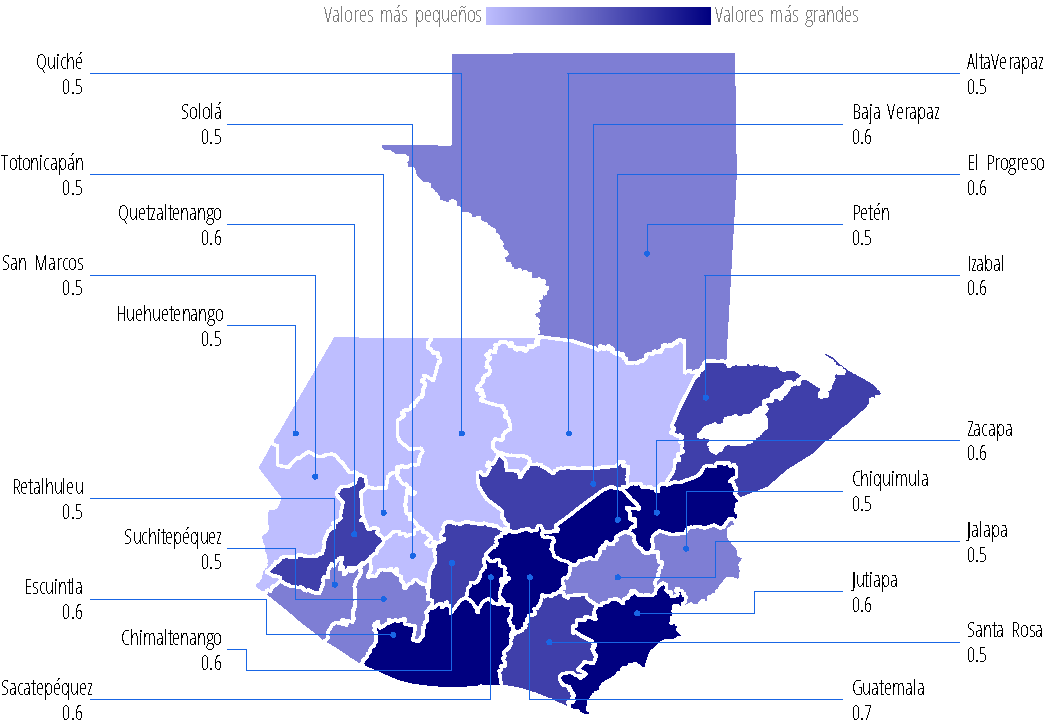
\includegraphics[width=52\cuadri]{graficas/1_11.pdf}}%
   	{%
   		Instituto Nacional de Estadística} %
 
 
 
 
      %%%%%%%%%%%%%%%%%%%%%%%%%%%%%%%%%%11%%%%%%%%%%%%%%%%%%%%%%%%
      
      \cajota{%
      	Calidad de la vivienda en los departamentos}%
      {%
  La vivienda formal es una de las necesidades básicas. Para el cálculo se incluyen las variables asociadas con los materiales de construcción utilizados en el piso, paredes y techo. 
   
   En el 2011, los departamentos donde más de la mitad de los hogares en el área rural tenían esta necesidad básica insatisfecha fueron Alta Verapaz (77.2\%), Quiché (70.2\%) Jalapa (70.1\%), Chiquimula (60.6\%), Totonicapán (59.0\%), Huehuetenango (56.2\%),  Petén (54.4\%) y Baja Verapaz (54.0\%). \textollamada[*]{Es un método directo para identificar carencias críticas en una población y caracterizar la pobreza. Toma datos disponibles de los censos de población y encuestas de condiciones de vida. La fuente más frecuente para la toma de esta información es la Encuesta Nacional de Condiciones de Vida.} }%
      {%
      	Proporción de hogares del área rural que no habitan en una vivienda formal
      } %
      {%
      	Por departamento, año 2011, en porcentaje} %
      {%
      	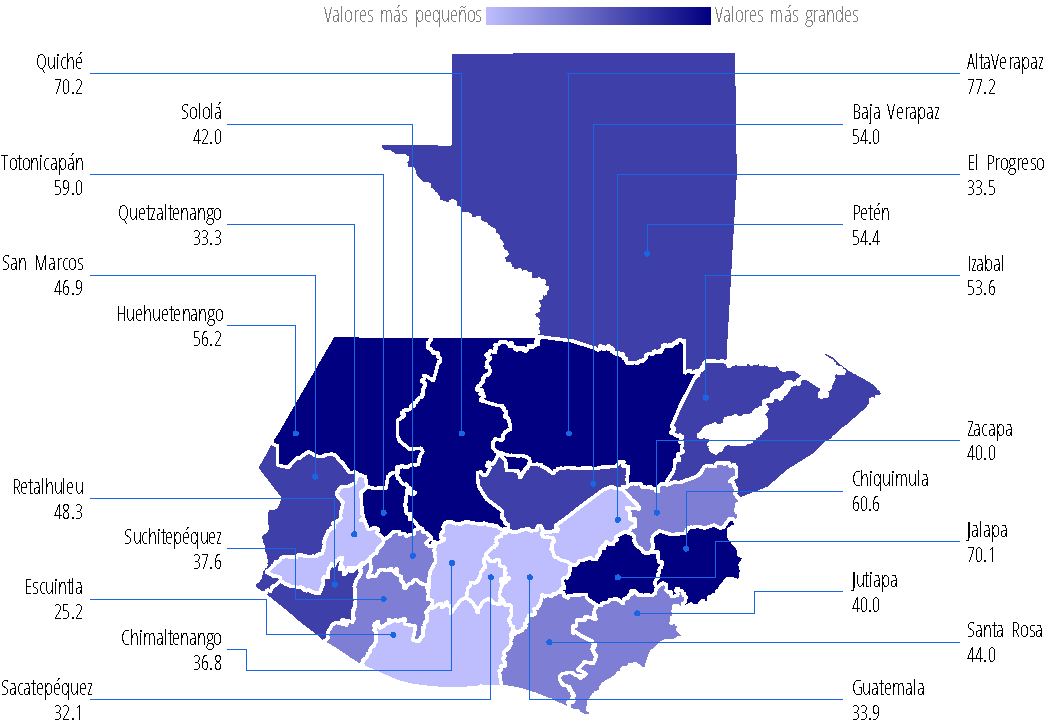
\includegraphics[width=52\cuadri]{graficas/1_12.pdf}}%
      {%
      	Instituto Nacional de Estadística} %
      
      
        %%%%%%%%%%%%%%%%%%%%%%%%%%%%%%%%%%12%%%%%%%%%%%%%%%%%%%%%%%%
        
        \cajota{%
        	Hogares que viven en hacinamiento en los departamentos}%
        {% 
        El hacinamiento toma las variables de la Encuesta Nacional de Condiciones de Vida que recogen información sobre el número de personas en el hogar y el número de cuartos de la vivienda.
        
        Los departamentos con mayor porcentaje de hogares en el área rural que vivían en hacinamiento en el 2011 fueron: Alta Verapaz (64.8\%), Quiché (59.9\%), Huehuetenango (54.6\%), San Marcos (54.6\%), Suchitepéquez (52.7\%), Izabal (52.5\%), Petén (51.4\%), Jalapa (51.4\%). }%
        {%
        Proporción de hogares del área rural que viven en hacinamiento
        } %
        {%
        	Por departamento, año 2011, en porcentaje} %
        {%
        	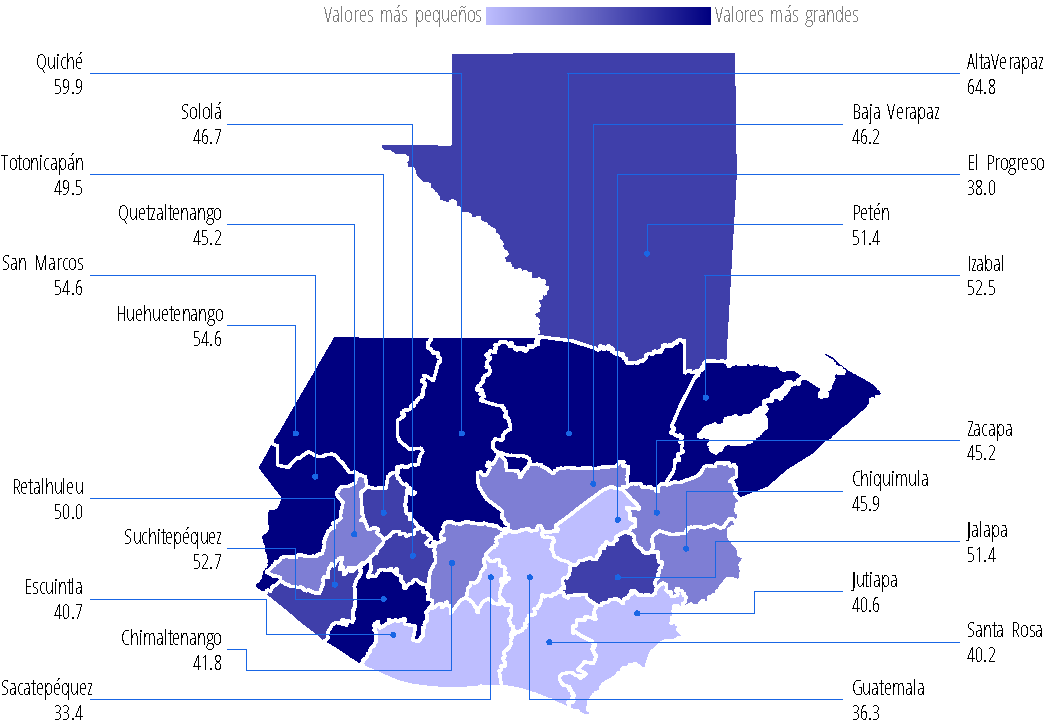
\includegraphics[width=52\cuadri]{graficas/1_13.pdf}}%
        {%
        	Instituto Nacional de Estadística} %
        
        
          
          %%%%%%%%%%%%%%%%%%%%%%%%%%%%%%%%%%13%%%%%%%%%%%%%%%%%%%%%%%%
          
          \cajota{%
          	Acceso a agua}%
          {%
         El acceso y/o disponibilidad de agua potable se encuentra en las necesidades básicas de acceso a servicios sanitarios.  Se toma de las variables de las Encovi que recogen información sobre la fuente de abastecimiento de agua en la vivienda.
         
         Para el 2011, los departamentos en los cuales más del 50\% de los hogares rurales no contaban con la disponibilidad de agua potable fuen Alta Verapaz y Retalhuleu.}%
          {%
          	Proporción de hogares del área rural que no poseían acceso a agua potable
          } %
          {%
          Por departamento, año 2011, en porcentaje} %
          {%
          	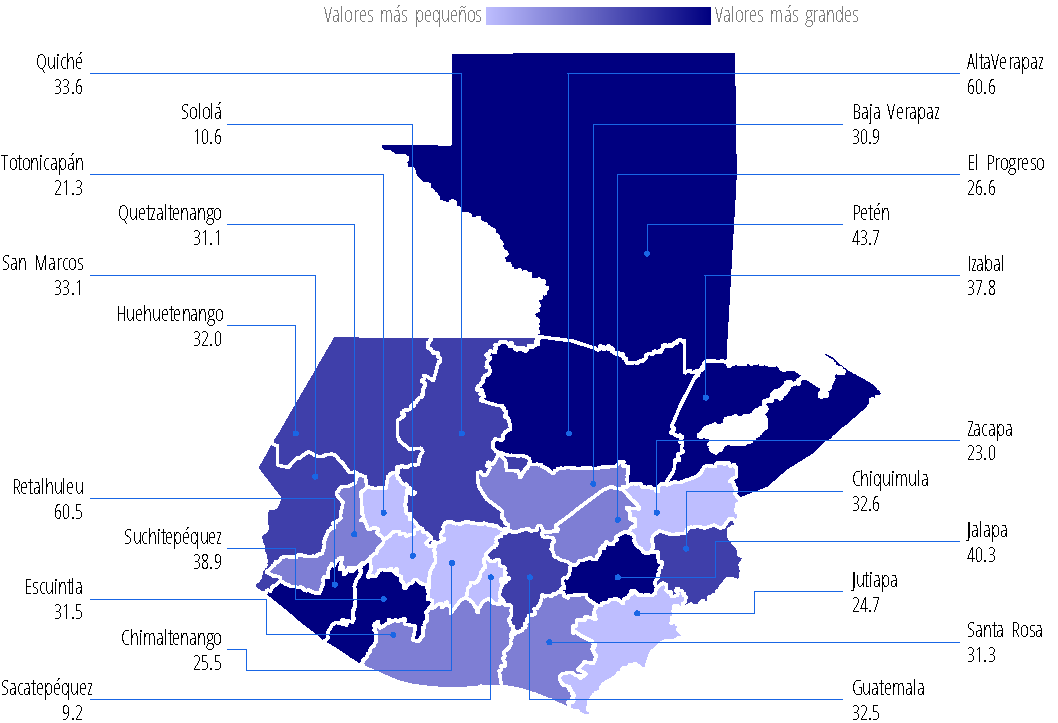
\includegraphics[width=52\cuadri]{graficas/1_14.pdf}}%
          {%
          	Instituto Nacional de Estadística} %
          
          
                    %%%%%%%%%%%%%%%%%%%%%%%%%%%%%%%%%%14%%%%%%%%%%%%%%%%%%%%%%%%
                    
                    \cajota{%
                    Acceso a servicios de saneamiento}%
                    {%
Esta necesidad básica clasificada en el acceso a servicios sanitarios, tomas las variables de la Encuesta Nacional de Condiciones de Vida que recoge datos sobre la disponibilidad de servicios sanitarios y sistemas de eliminación de excretas.

Para el 2011, el 40.4\% de los hogares rurales en Chiquimula no contaban con acceso a servicios de saneamiento y en Jutiapa, Petén y Jalapa, 3 de cada 10 hogares del área rural también carecían de este servicio.   }%
                    {%
                    	Proporción de hogares del área rural sin acceso a servicios de saneamiento }
                    {%
                    	Por departamento, año 2011, en porcentaje} %
                    {%
                    	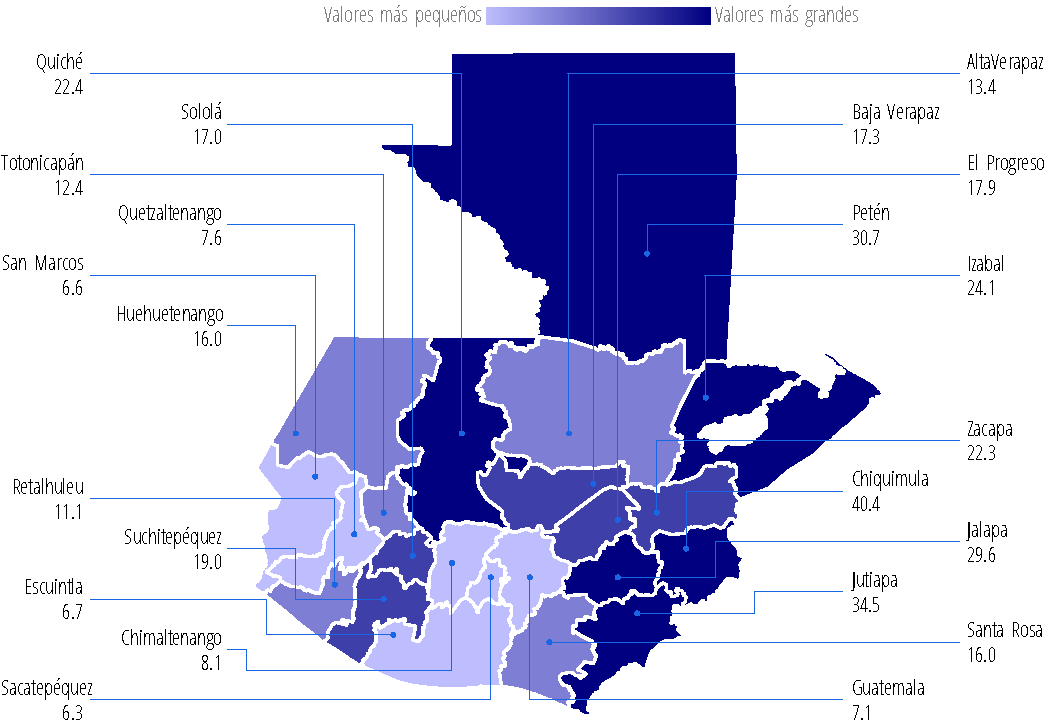
\includegraphics[width=52\cuadri]{graficas/1_15.pdf}}%
                    {%
                    	Instituto Nacional de Estadística} %

                  
                     %%%%%%%%%%%%%%%%%%%%%%%%%%%%%%%%%%18%%%%%%%%%%%%%%%%%%%%%%%%
                     
                     \cajota{%
                     	Pobreza total }%
                     {%
                  Según la Encuesta Nacional de Condiciones de Vida 2014, los departamentos con mayor incidencia de pobreza (que incluye la pobreza extrema y la no extrema) fueron Alta Verapaz con el 83.1\%, Sololá con 80.9\%, Totonicapán 77.5\% y Quiché con 74.7\%. }%
                     {%
                     	Pobreza total
                     } %
                     {%
                     Por departamento, año 2014, en porcentaje} %
                     {%
                     	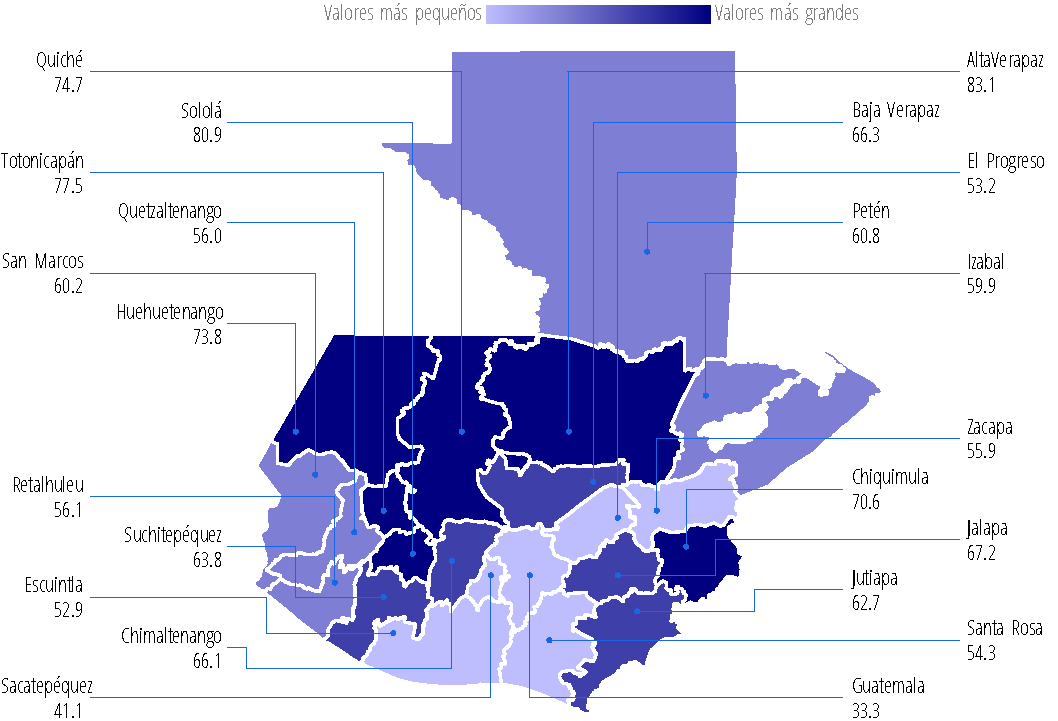
\includegraphics[width=52\cuadri]{graficas/1_19.pdf}}%
                     {%
                     	INE, ENCOVI 2014} %
                     
                    %%%%%%%%%%%%%%%%%%%%%%%%%%%%%%%%%%16%%%%%%%%%%%%%%%%%%%%%%%%
                    
                    \cajota{%
                    	Pobreza total rural}%
                    {%
                    Los departamentos donde 8 de cada 10 personas que habitaban en áreas rurales estaban en condiciones de pobreza (extremo o no extremo) fueron Alta Verapaz, Quiché, Totonicapán y Sololá}%
                    {%
                    	Pobreza total rural
                    } %
                    {%
                    Por departamento, año 2014, en porcentaje} %
                    {%
                    	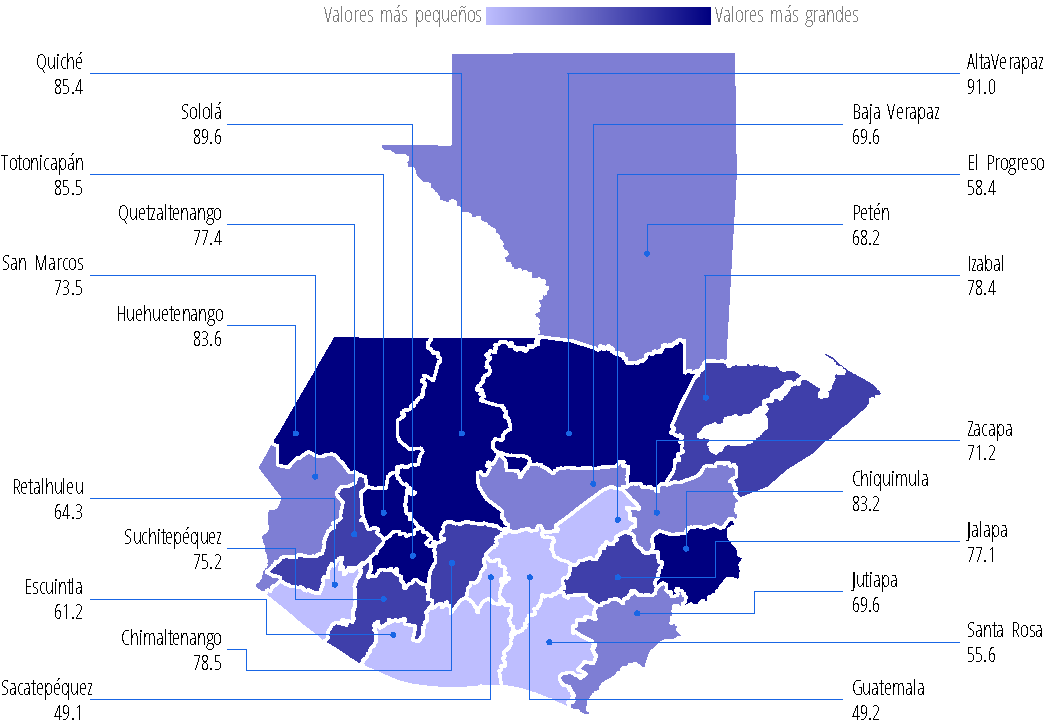
\includegraphics[width=52\cuadri]{graficas/1_17.pdf}}%
                    {%
                    	INE, ENCOVI 2014} %
                    %%%%%%%%%%%%%%%%%%%%%%%%%%%%%%%%%%17%%%%%%%%%%%%%%%%%%%%%%%%
                    
                    \cajota{%
                    	Pobreza extrema }%
                    {%
                   La pobreza extrema a nivel departamental  }%
                    {%
                    El departamento con la mayor incidencia de pobreza extrema fue Alta Verapaz (53.6\%).
                    } %
                    {%
                    	República de Guatemala, por departamentos año 2014, en porcentaje} %
                    {%
                    	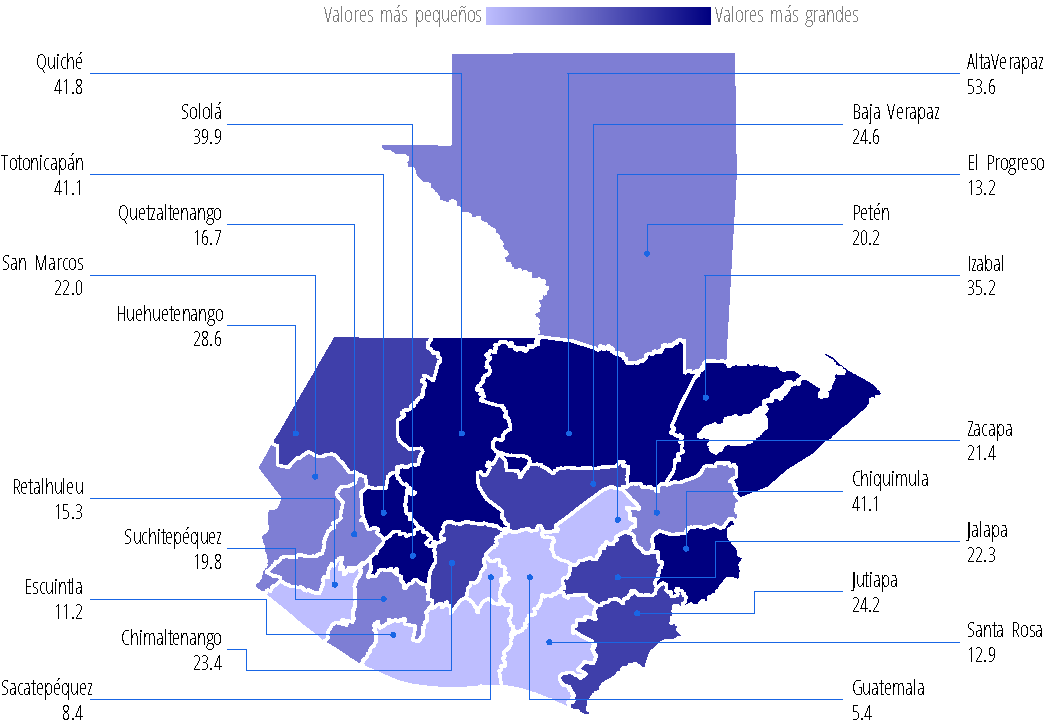
\includegraphics[width=52\cuadri]{graficas/1_18.pdf}}%
                    {%
                    	INE, ENCOVI 2014} %
                    
                     %%%%%%%%%%%%%%%%%%%%%%%%%%%%%%%%%%15%%%%%%%%%%%%%%%%%%%%%%%%
                     
                     \cajota{%
                     	Pobreza extrema rural}%
                     {%
                     	El análisis de las personas que habitan en áreas rurales y desagregarlos según su nivel de pobreza, muestra que el 50.4\% de los habitantes en áreas rurales en Sololá estaban debajo de la línea de pobreza extrema, así también Izabal (52.1\%), 52.9\% en Totonicapán, 54.2\% en Chiquimula, 57.9\% en Alta Verapaz, que fueron los departamentos con mayor incidencia en el 2014.
                     	
                     	En Alta Verapaz la incidencia de pobreza extrema en las áreas rurales es mayor que la incidencia departamental en 4.3 puntos porcentuales.}%
                     {%
                     	Pobreza extrema rural por departamentos
                     } %
                     {%
                     	Por departamento, año 2014, en porcentaje} %
                     {%
                     	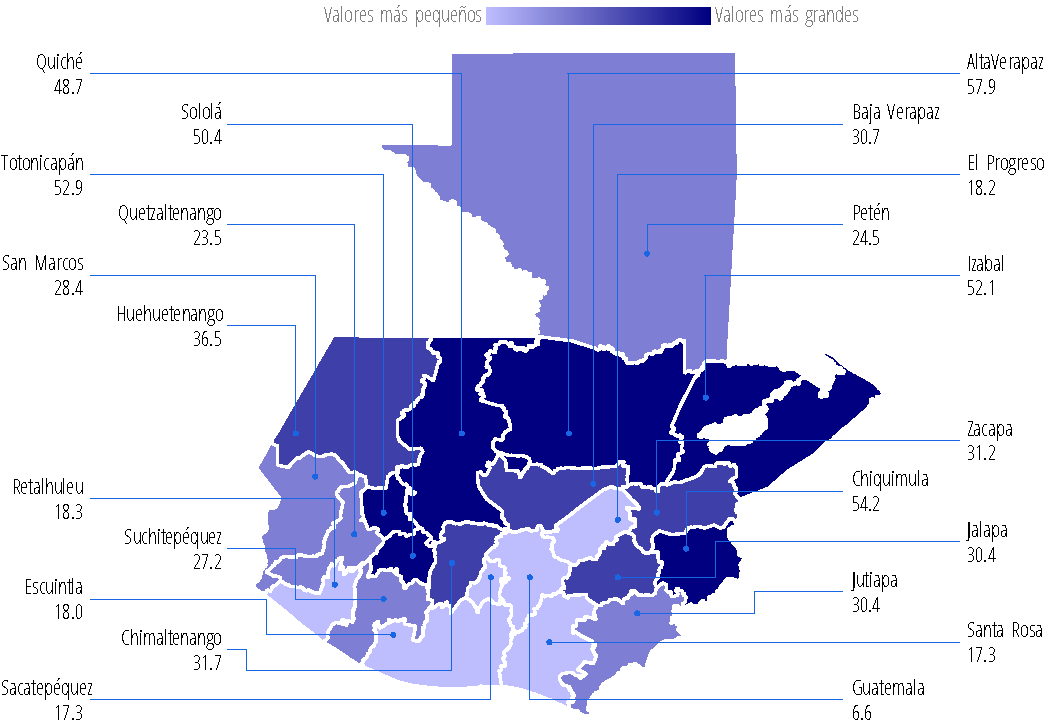
\includegraphics[width=52\cuadri]{graficas/1_16.pdf}}%
                     {%
                     	INE, ENCOVI 2014} %
         
 %%%%%%%%%%%%%%%%%%%%%%%%%%%%%%%%%%19%%%%%%%%%%%%%%%%%%%%%%%%
 
 \cajita{%
 	PET }%
 {%
 De acuerdo a las encuestas nacionales de empleo e ingresos, desde el 2011 hasta 2-2014\llamada, la evolución de la población en edad de trabajar muestra que para el 2014 había 10.5 millones de personas mayores de 14 años, número que aumentó en un 6.1\% respecto al 2013.
 
 \textollamada{El número 2 que antecede al año indica que la encuesta se realizó en el segundo semestre, aplicable a los años 2013 y 2014.}}%
 {%
 	Población en edad de trabajar} %
 {%
 	República de Guatemala, serie histórica por ENEI, en número de personas} %
 {%
 	\begin{tikzpicture}[x=1pt,y=1pt]  % Created by tikzDevice version 0.9 on 2016-03-03 00:54:40
% !TEX encoding = UTF-8 Unicode
\definecolor{fillColor}{RGB}{255,255,255}
\path[use as bounding box,fill=fillColor,fill opacity=0.00] (0,0) rectangle (289.08,198.74);
\begin{scope}
\path[clip] (  0.00,  0.00) rectangle (289.08,198.74);

\path[] (  0.00,  0.00) rectangle (289.08,198.74);
\end{scope}
\begin{scope}
\path[clip] (  0.00,  0.00) rectangle (289.08,198.74);

\path[] ( 25.76, 15.61) rectangle (280.54,191.48);

\path[] ( 25.76, 31.48) --
	(280.54, 31.48);

\path[] ( 25.76, 74.96) --
	(280.54, 74.96);

\path[] ( 25.76,118.43) --
	(280.54,118.43);

\path[] ( 25.76,161.90) --
	(280.54,161.90);

\path[] ( 25.76, 53.22) --
	(280.54, 53.22);

\path[] ( 25.76, 96.69) --
	(280.54, 96.69);

\path[] ( 25.76,140.16) --
	(280.54,140.16);

\path[] ( 25.76,183.64) --
	(280.54,183.64);

\path[] ( 62.15, 15.61) --
	( 62.15,191.48);

\path[] (122.82, 15.61) --
	(122.82,191.48);

\path[] (183.48, 15.61) --
	(183.48,191.48);

\path[] (244.15, 15.61) --
	(244.15,191.48);
\definecolor{drawColor}{RGB}{0,0,255}

\path[draw=drawColor,line width= 1.7pt,line join=round] ( 62.15, 60.50) --
	(122.82, 99.42) --
	(183.48,131.03) --
	(244.15,183.49);
\definecolor{drawColor}{RGB}{0,0,0}

\node[text=drawColor,anchor=base,inner sep=0pt, outer sep=0pt, scale=  1.02] at ( 62.15, 48.59) {9,083,763};

\node[text=drawColor,anchor=base east,inner sep=0pt, outer sep=0pt, scale=  1.02] at (115.67, 99.42) {9,531,370};

\node[text=drawColor,anchor=base east,inner sep=0pt, outer sep=0pt, scale=  1.02] at (176.34,131.03) {9,894,951};

\node[text=drawColor,anchor=base,inner sep=0pt, outer sep=0pt, scale=  1.02] at (244.15,187.46) {10,498,289};

\path[draw=drawColor,line width= 0.1pt,line join=round] ( 25.76, 23.61) -- (280.54, 23.61);

\path[] ( 25.76, 15.61) rectangle (280.54,191.48);
\end{scope}
\begin{scope}
\path[clip] (  0.00,  0.00) rectangle (289.08,198.74);

\path[] ( 25.76, 15.61) --
	( 25.76,191.48);
\end{scope}
\begin{scope}
\path[clip] (  0.00,  0.00) rectangle (289.08,198.74);
\definecolor{drawColor}{RGB}{255,255,255}

\node[text=drawColor,text opacity=0.00,anchor=base east,inner sep=0pt, outer sep=0pt, scale=  1.00] at ( 20.81, 49.31) {9000000};

\node[text=drawColor,text opacity=0.00,anchor=base east,inner sep=0pt, outer sep=0pt, scale=  1.00] at ( 20.81, 92.78) {9500000};

\node[text=drawColor,text opacity=0.00,anchor=base east,inner sep=0pt, outer sep=0pt, scale=  1.00] at ( 20.81,136.26) {10000000};

\node[text=drawColor,text opacity=0.00,anchor=base east,inner sep=0pt, outer sep=0pt, scale=  1.00] at ( 20.81,179.73) {10500000};
\end{scope}
\begin{scope}
\path[clip] (  0.00,  0.00) rectangle (289.08,198.74);

\path[] ( 23.01, 53.22) --
	( 25.76, 53.22);

\path[] ( 23.01, 96.69) --
	( 25.76, 96.69);

\path[] ( 23.01,140.16) --
	( 25.76,140.16);

\path[] ( 23.01,183.64) --
	( 25.76,183.64);
\end{scope}
\begin{scope}
\path[clip] (  0.00,  0.00) rectangle (289.08,198.74);

\path[] ( 25.76, 15.61) --
	(280.54, 15.61);
\end{scope}
\begin{scope}
\path[clip] (  0.00,  0.00) rectangle (289.08,198.74);

\path[] ( 62.15, 12.86) --
	( 62.15, 15.61);

\path[] (122.82, 12.86) --
	(122.82, 15.61);

\path[] (183.48, 12.86) --
	(183.48, 15.61);

\path[] (244.15, 12.86) --
	(244.15, 15.61);
\end{scope}
\begin{scope}
\path[clip] (  0.00,  0.00) rectangle (289.08,198.74);
\definecolor{drawColor}{RGB}{0,0,0}

\node[text=drawColor,anchor=base,inner sep=0pt, outer sep=0pt, scale=  1.00] at ( 62.15,  2.85) {2011};

\node[text=drawColor,anchor=base,inner sep=0pt, outer sep=0pt, scale=  1.00] at (122.82,  2.85) {2012};

\node[text=drawColor,anchor=base,inner sep=0pt, outer sep=0pt, scale=  1.00] at (183.48,  2.85) {2013};

\node[text=drawColor,anchor=base,inner sep=0pt, outer sep=0pt, scale=  1.00] at (244.15,  2.85) {2014};
\end{scope}
  \end{tikzpicture}}%
 {%
 	ENEI 2011, 2012, 2-2013, 2-2014} % 
 
 
  %%%%%%%%%%%%%%%%%%%%%%%%%%%%%%%%%%20%%%%%%%%%%%%%%%%%%%%%%%%
 
 \cajita{%
 	PEA }%
 {%
 De la población en edad de trabajar, en el 2014 el 60.2\% estaba activo, lo que significa que estaba trabajando o buscando trabajo.
 }%
 {%
 	Población económicamente activa} %
 {%
 	República de Guatemala, serie histórica por ENEI, en número de personas} %
 {%
 	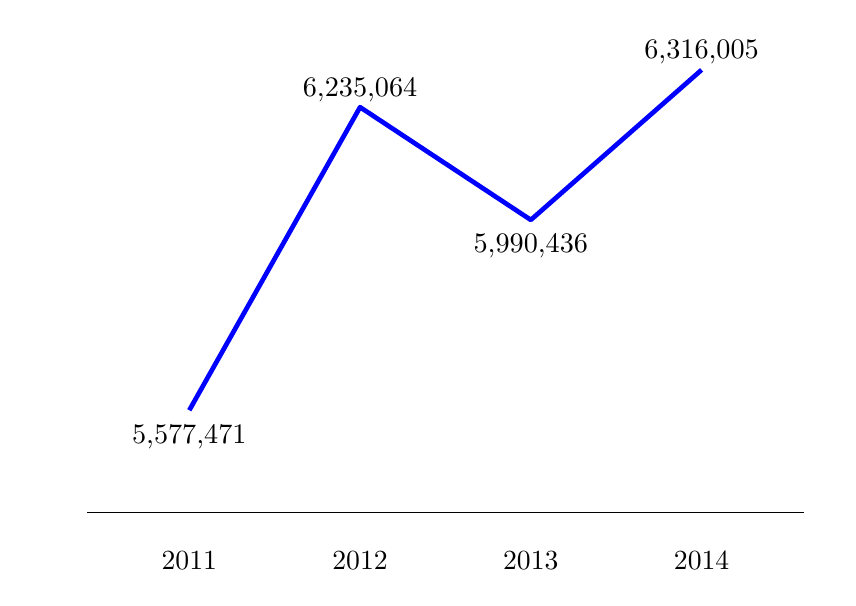
\begin{tikzpicture}[x=1pt,y=1pt]  % Created by tikzDevice version 0.9 on 2016-03-03 02:00:13
% !TEX encoding = UTF-8 Unicode
\definecolor{fillColor}{RGB}{255,255,255}
\path[use as bounding box,fill=fillColor,fill opacity=0.00] (0,0) rectangle (289.08,198.74);
\begin{scope}
\path[clip] (  0.00,  0.00) rectangle (289.08,198.74);

\path[] (  0.00,  0.00) rectangle (289.08,198.74);
\end{scope}
\begin{scope}
\path[clip] (  0.00,  0.00) rectangle (289.08,198.74);

\path[] ( 21.38, 15.61) rectangle (280.54,191.48);

\path[] ( 21.38, 26.79) --
	(280.54, 26.79);

\path[] ( 21.38, 68.42) --
	(280.54, 68.42);

\path[] ( 21.38,110.05) --
	(280.54,110.05);

\path[] ( 21.38,151.68) --
	(280.54,151.68);

\path[] ( 21.38, 47.60) --
	(280.54, 47.60);

\path[] ( 21.38, 89.23) --
	(280.54, 89.23);

\path[] ( 21.38,130.87) --
	(280.54,130.87);

\path[] ( 21.38,172.50) --
	(280.54,172.50);

\path[] ( 58.40, 15.61) --
	( 58.40,191.48);

\path[] (120.11, 15.61) --
	(120.11,191.48);

\path[] (181.81, 15.61) --
	(181.81,191.48);

\path[] (243.52, 15.61) --
	(243.52,191.48);
\definecolor{drawColor}{RGB}{0,0,255}

\path[draw=drawColor,line width= 1.7pt,line join=round] ( 58.40, 60.50) --
	(120.11,170.01) --
	(181.81,129.27) --
	(243.52,183.49);
\definecolor{drawColor}{RGB}{0,0,0}

\node[text=drawColor,anchor=base,inner sep=0pt, outer sep=0pt, scale=  1.02] at ( 58.40, 48.59) {5,577,471};

\node[text=drawColor,anchor=base,inner sep=0pt, outer sep=0pt, scale=  1.02] at (120.11,173.98) {6,235,064};

\node[text=drawColor,anchor=base,inner sep=0pt, outer sep=0pt, scale=  1.02] at (181.81,117.36) {5,990,436};

\node[text=drawColor,anchor=base,inner sep=0pt, outer sep=0pt, scale=  1.02] at (243.52,187.46) {6,316,005};

\path[draw=drawColor,line width= 0.1pt,line join=round] ( 21.38, 23.61) -- (280.54, 23.61);

\path[] ( 21.38, 15.61) rectangle (280.54,191.48);
\end{scope}
\begin{scope}
\path[clip] (  0.00,  0.00) rectangle (289.08,198.74);

\path[] ( 21.38, 15.61) --
	( 21.38,191.48);
\end{scope}
\begin{scope}
\path[clip] (  0.00,  0.00) rectangle (289.08,198.74);
\definecolor{drawColor}{RGB}{255,255,255}

\node[text=drawColor,text opacity=0.00,anchor=base east,inner sep=0pt, outer sep=0pt, scale=  1.00] at ( 16.43, 43.69) {5500000};

\node[text=drawColor,text opacity=0.00,anchor=base east,inner sep=0pt, outer sep=0pt, scale=  1.00] at ( 16.43, 85.32) {5750000};

\node[text=drawColor,text opacity=0.00,anchor=base east,inner sep=0pt, outer sep=0pt, scale=  1.00] at ( 16.43,126.96) {6000000};

\node[text=drawColor,text opacity=0.00,anchor=base east,inner sep=0pt, outer sep=0pt, scale=  1.00] at ( 16.43,168.59) {6250000};
\end{scope}
\begin{scope}
\path[clip] (  0.00,  0.00) rectangle (289.08,198.74);

\path[] ( 18.63, 47.60) --
	( 21.38, 47.60);

\path[] ( 18.63, 89.23) --
	( 21.38, 89.23);

\path[] ( 18.63,130.87) --
	( 21.38,130.87);

\path[] ( 18.63,172.50) --
	( 21.38,172.50);
\end{scope}
\begin{scope}
\path[clip] (  0.00,  0.00) rectangle (289.08,198.74);

\path[] ( 21.38, 15.61) --
	(280.54, 15.61);
\end{scope}
\begin{scope}
\path[clip] (  0.00,  0.00) rectangle (289.08,198.74);

\path[] ( 58.40, 12.86) --
	( 58.40, 15.61);

\path[] (120.11, 12.86) --
	(120.11, 15.61);

\path[] (181.81, 12.86) --
	(181.81, 15.61);

\path[] (243.52, 12.86) --
	(243.52, 15.61);
\end{scope}
\begin{scope}
\path[clip] (  0.00,  0.00) rectangle (289.08,198.74);
\definecolor{drawColor}{RGB}{0,0,0}

\node[text=drawColor,anchor=base,inner sep=0pt, outer sep=0pt, scale=  1.00] at ( 58.40,  2.85) {2011};

\node[text=drawColor,anchor=base,inner sep=0pt, outer sep=0pt, scale=  1.00] at (120.11,  2.85) {2012};

\node[text=drawColor,anchor=base,inner sep=0pt, outer sep=0pt, scale=  1.00] at (181.81,  2.85) {2013};

\node[text=drawColor,anchor=base,inner sep=0pt, outer sep=0pt, scale=  1.00] at (243.52,  2.85) {2014};
\end{scope}
  \end{tikzpicture}}%
 {%
 	ENEI 2011, 2012, 2-2013, 2-2014} % 
 
 
  %%%%%%%%%%%%%%%%%%%%%%%%%%%%%%%%%%21%%%%%%%%%%%%%%%%%%%%%%%%
  
  \cajita{%
  	Población ocupada }%
  {%
 De la población económicamente activa en el 2014, el 97.1\% estaba ocupado.
 
 En términos relativos, la población ocupada del 2014 creció un 5.5\% respecto al 2013.}%
  {%
  	Población ocupada} %
  {%
  	República de Guatemala, serie histórica por ENEI, en número de personas} %
  {%
  	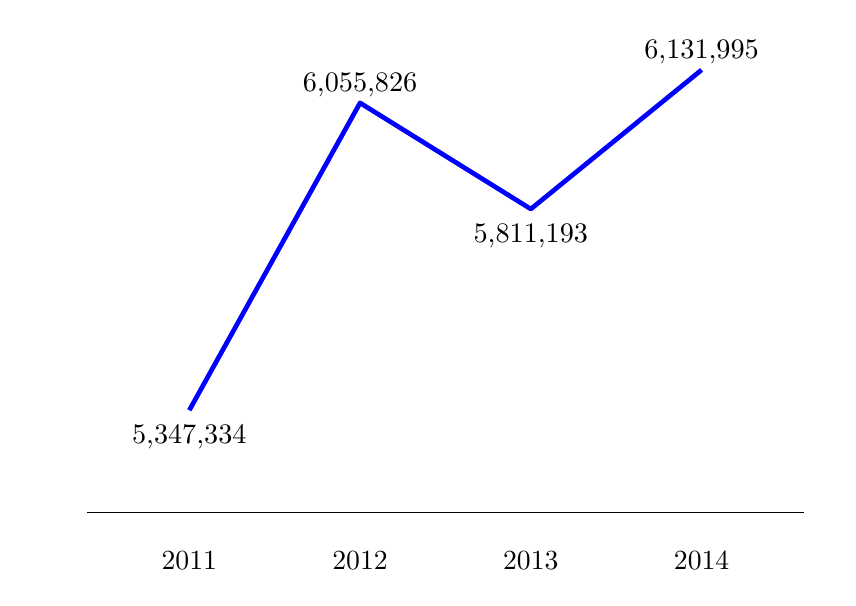
\begin{tikzpicture}[x=1pt,y=1pt]  % Created by tikzDevice version 0.9 on 2016-03-03 02:00:19
% !TEX encoding = UTF-8 Unicode
\definecolor{fillColor}{RGB}{255,255,255}
\path[use as bounding box,fill=fillColor,fill opacity=0.00] (0,0) rectangle (289.08,198.74);
\begin{scope}
\path[clip] (  0.00,  0.00) rectangle (289.08,198.74);

\path[] (  0.00,  0.00) rectangle (289.08,198.74);
\end{scope}
\begin{scope}
\path[clip] (  0.00,  0.00) rectangle (289.08,198.74);

\path[] ( 21.38, 15.61) rectangle (280.54,191.48);

\path[] ( 21.38, 25.65) --
	(280.54, 25.65);

\path[] ( 21.38, 64.84) --
	(280.54, 64.84);

\path[] ( 21.38,104.02) --
	(280.54,104.02);

\path[] ( 21.38,143.21) --
	(280.54,143.21);

\path[] ( 21.38,182.39) --
	(280.54,182.39);

\path[] ( 21.38, 45.25) --
	(280.54, 45.25);

\path[] ( 21.38, 84.43) --
	(280.54, 84.43);

\path[] ( 21.38,123.62) --
	(280.54,123.62);

\path[] ( 21.38,162.80) --
	(280.54,162.80);

\path[] ( 58.40, 15.61) --
	( 58.40,191.48);

\path[] (120.11, 15.61) --
	(120.11,191.48);

\path[] (181.81, 15.61) --
	(181.81,191.48);

\path[] (243.52, 15.61) --
	(243.52,191.48);
\definecolor{drawColor}{RGB}{0,0,255}

\path[draw=drawColor,line width= 1.7pt,line join=round] ( 58.40, 60.50) --
	(120.11,171.55) --
	(181.81,133.21) --
	(243.52,183.49);
\definecolor{drawColor}{RGB}{0,0,0}

\node[text=drawColor,anchor=base,inner sep=0pt, outer sep=0pt, scale=  1.02] at ( 58.40, 48.59) {5,347,334};

\node[text=drawColor,anchor=base,inner sep=0pt, outer sep=0pt, scale=  1.02] at (120.11,175.52) {6,055,826};

\node[text=drawColor,anchor=base,inner sep=0pt, outer sep=0pt, scale=  1.02] at (181.81,121.29) {5,811,193};

\node[text=drawColor,anchor=base,inner sep=0pt, outer sep=0pt, scale=  1.02] at (243.52,187.46) {6,131,995};

\path[draw=drawColor,line width= 0.1pt,line join=round] ( 21.38, 23.61) -- (280.54, 23.61);

\path[] ( 21.38, 15.61) rectangle (280.54,191.48);
\end{scope}
\begin{scope}
\path[clip] (  0.00,  0.00) rectangle (289.08,198.74);

\path[] ( 21.38, 15.61) --
	( 21.38,191.48);
\end{scope}
\begin{scope}
\path[clip] (  0.00,  0.00) rectangle (289.08,198.74);
\definecolor{drawColor}{RGB}{255,255,255}

\node[text=drawColor,text opacity=0.00,anchor=base east,inner sep=0pt, outer sep=0pt, scale=  1.00] at ( 16.43, 41.34) {5250000};

\node[text=drawColor,text opacity=0.00,anchor=base east,inner sep=0pt, outer sep=0pt, scale=  1.00] at ( 16.43, 80.52) {5500000};

\node[text=drawColor,text opacity=0.00,anchor=base east,inner sep=0pt, outer sep=0pt, scale=  1.00] at ( 16.43,119.71) {5750000};

\node[text=drawColor,text opacity=0.00,anchor=base east,inner sep=0pt, outer sep=0pt, scale=  1.00] at ( 16.43,158.89) {6000000};
\end{scope}
\begin{scope}
\path[clip] (  0.00,  0.00) rectangle (289.08,198.74);

\path[] ( 18.63, 45.25) --
	( 21.38, 45.25);

\path[] ( 18.63, 84.43) --
	( 21.38, 84.43);

\path[] ( 18.63,123.62) --
	( 21.38,123.62);

\path[] ( 18.63,162.80) --
	( 21.38,162.80);
\end{scope}
\begin{scope}
\path[clip] (  0.00,  0.00) rectangle (289.08,198.74);

\path[] ( 21.38, 15.61) --
	(280.54, 15.61);
\end{scope}
\begin{scope}
\path[clip] (  0.00,  0.00) rectangle (289.08,198.74);

\path[] ( 58.40, 12.86) --
	( 58.40, 15.61);

\path[] (120.11, 12.86) --
	(120.11, 15.61);

\path[] (181.81, 12.86) --
	(181.81, 15.61);

\path[] (243.52, 12.86) --
	(243.52, 15.61);
\end{scope}
\begin{scope}
\path[clip] (  0.00,  0.00) rectangle (289.08,198.74);
\definecolor{drawColor}{RGB}{0,0,0}

\node[text=drawColor,anchor=base,inner sep=0pt, outer sep=0pt, scale=  1.00] at ( 58.40,  2.85) {2011};

\node[text=drawColor,anchor=base,inner sep=0pt, outer sep=0pt, scale=  1.00] at (120.11,  2.85) {2012};

\node[text=drawColor,anchor=base,inner sep=0pt, outer sep=0pt, scale=  1.00] at (181.81,  2.85) {2013};

\node[text=drawColor,anchor=base,inner sep=0pt, outer sep=0pt, scale=  1.00] at (243.52,  2.85) {2014};
\end{scope}
  \end{tikzpicture}}%
  {%
  	ENEI 2014, 2013, 2012 y 2011} %  
  
  
  
  %%%%%%%%%%%%%%%%%%%%%%%%%%%%%%%%%%22%%%%%%%%%%%%%%%%%%%%%%%%
  
  \cajita{%
  	Participación por dominio}%
  {%
La participación de la población ocupada se realiza respecto a la población en edad de trabajar.

Para el año 2014, en el dominio urbano metropolitano la tasa de participación de la población ocupada era la mayor, con el 62.4\%. 

En el resto urbano, casi 6 de cada 10 personas en edad de trabajar estaban ocupados, al igual que en el dominio rural nacional. }%
  {%
  	Tasa de participación de la población ocupada según dominio de estudio} %
  {%
  	República de Guatemala, año 2014, en porcentaje} %
  {%
  	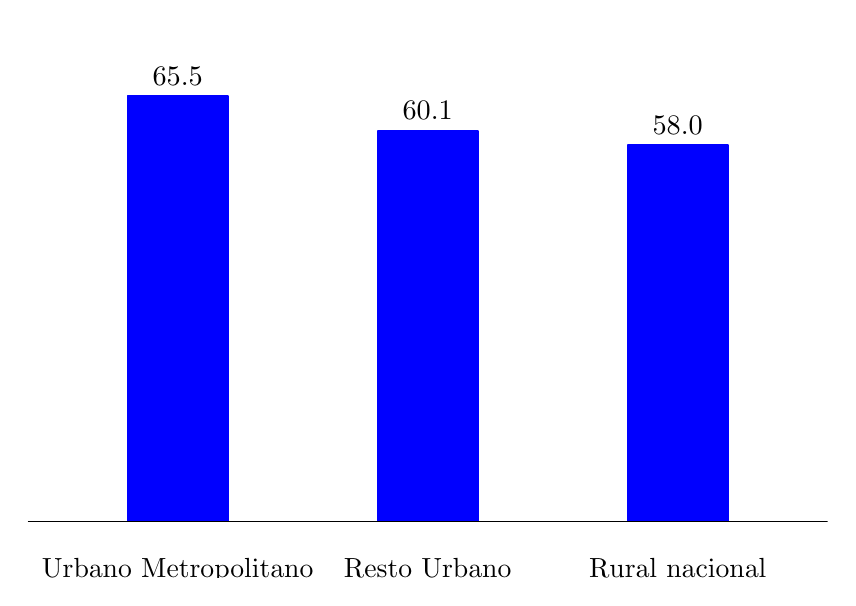
\begin{tikzpicture}[x=1pt,y=1pt]  % Created by tikzDevice version 0.9 on 2016-03-03 02:00:22
% !TEX encoding = UTF-8 Unicode
\definecolor{fillColor}{RGB}{255,255,255}
\path[use as bounding box,fill=fillColor,fill opacity=0.00] (0,0) rectangle (289.08,198.74);
\begin{scope}
\path[clip] (  0.00,  0.00) rectangle (289.08,198.74);

\path[] (  0.00,  0.00) rectangle (289.08,198.74);
\end{scope}
\begin{scope}
\path[clip] (  0.00,  0.00) rectangle (289.08,198.74);

\path[] (  0.00, 12.77) rectangle (289.08,181.67);

\path[] ( 54.20, 12.77) --
	( 54.20,181.67);

\path[] (144.54, 12.77) --
	(144.54,181.67);

\path[] (234.88, 12.77) --
	(234.88,181.67);
\definecolor{drawColor}{RGB}{0,0,255}
\definecolor{fillColor}{RGB}{0,0,255}

\path[draw=drawColor,line width= 0.6pt,line join=round,fill=fillColor] ( 36.13, 20.44) rectangle ( 72.27,173.99);

\path[draw=drawColor,line width= 0.6pt,line join=round,fill=fillColor] (126.47, 20.44) rectangle (162.61,161.43);

\path[draw=drawColor,line width= 0.6pt,line join=round,fill=fillColor] (216.81, 20.44) rectangle (252.95,156.30);
\definecolor{drawColor}{RGB}{0,0,0}

\path[draw=drawColor,line width= 0.1pt,line join=round] (  0.00, 20.44) -- (289.08, 20.44);

\node[text=drawColor,anchor=base,inner sep=0pt, outer sep=0pt, scale=  1.02] at ( 54.20,177.96) {65.5};

\node[text=drawColor,anchor=base,inner sep=0pt, outer sep=0pt, scale=  1.02] at (144.54,165.40) {60.1};

\node[text=drawColor,anchor=base,inner sep=0pt, outer sep=0pt, scale=  1.02] at (234.88,160.27) {58.0};

\path[] (  0.00, 12.77) rectangle (289.08,181.67);
\end{scope}
\begin{scope}
\path[clip] (  0.00,  0.00) rectangle (289.08,198.74);

\path[] (  0.00, 12.77) --
	(289.08, 12.77);
\end{scope}
\begin{scope}
\path[clip] (  0.00,  0.00) rectangle (289.08,198.74);

\path[] ( 54.20, 10.02) --
	( 54.20, 12.77);

\path[] (144.54, 10.02) --
	(144.54, 12.77);

\path[] (234.88, 10.02) --
	(234.88, 12.77);
\end{scope}
\begin{scope}
\path[clip] (  0.00,  0.00) rectangle (289.08,198.74);
\definecolor{drawColor}{RGB}{0,0,0}

\node[text=drawColor,anchor=base,inner sep=0pt, outer sep=0pt, scale=  1.00] at ( 54.20, -0.00) {Urbano Metropolitano};

\node[text=drawColor,anchor=base,inner sep=0pt, outer sep=0pt, scale=  1.00] at (144.54, -0.00) {Resto Urbano};

\node[text=drawColor,anchor=base,inner sep=0pt, outer sep=0pt, scale=  1.00] at (234.88, -0.00) {Rural nacional};
\end{scope}
  \end{tikzpicture}}%
  {%
  	ENEI 2014} %  
  
  
 %%%%%%%%%%%%%%%%%%%%%%%%%%%%%%%%%%23%%%%%%%%%%%%%%%%%%%%%%%%
 
 \cajita{%
 	Tasa de participación según sexo}%
 {%
 La tasa de participación nacional de la población ocupada en el 2014 fue de 58.4\%.
 
 Al desagregar esto por sexo, estaban ocupados 8 de cada 10 hombres en edad de trabajar y casi 4 de cada 10 mujeres en edad de trabajar.}%
 {%
 	Tasa de participación de la población ocupada según sexo} %
 {%
 	República de Guatemala, año 2014, en porcentaje} %
 {%
 	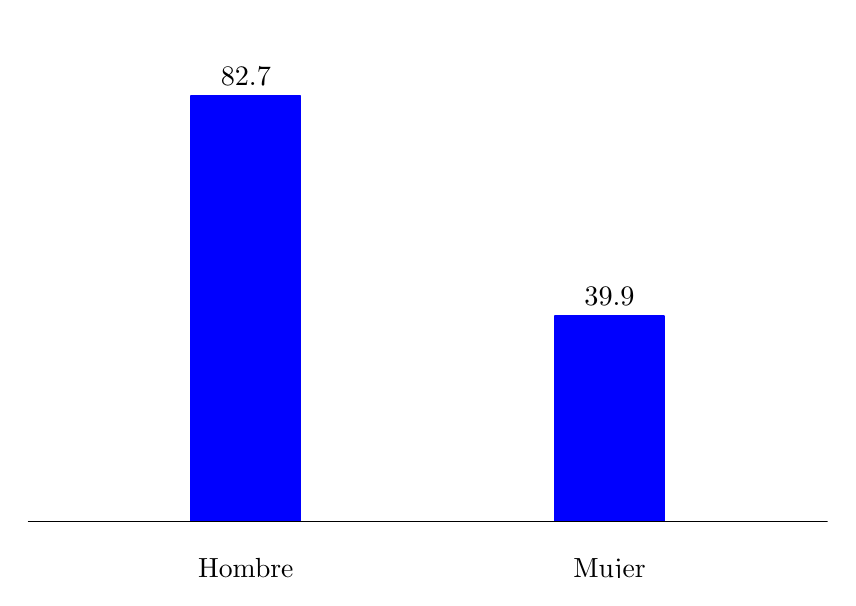
\begin{tikzpicture}[x=1pt,y=1pt]  % Created by tikzDevice version 0.9 on 2016-03-03 02:05:06
% !TEX encoding = UTF-8 Unicode
\definecolor{fillColor}{RGB}{255,255,255}
\path[use as bounding box,fill=fillColor,fill opacity=0.00] (0,0) rectangle (289.08,198.74);
\begin{scope}
\path[clip] (  0.00,  0.00) rectangle (289.08,198.74);

\path[] (  0.00,  0.00) rectangle (289.08,198.74);
\end{scope}
\begin{scope}
\path[clip] (  0.00,  0.00) rectangle (289.08,198.74);

\path[] (  0.00, 12.77) rectangle (289.08,181.67);

\path[] ( 78.84, 12.77) --
	( 78.84,181.67);

\path[] (210.24, 12.77) --
	(210.24,181.67);
\definecolor{drawColor}{RGB}{0,0,255}
\definecolor{fillColor}{RGB}{0,0,255}

\path[draw=drawColor,line width= 0.6pt,line join=round,fill=fillColor] ( 59.13, 20.44) rectangle ( 98.55,173.99);

\path[draw=drawColor,line width= 0.6pt,line join=round,fill=fillColor] (190.53, 20.44) rectangle (229.95, 94.54);
\definecolor{drawColor}{RGB}{0,0,0}

\path[draw=drawColor,line width= 0.1pt,line join=round] (  0.00, 20.44) -- (289.08, 20.44);

\node[text=drawColor,anchor=base,inner sep=0pt, outer sep=0pt, scale=  1.02] at ( 78.84,177.96) {82.7};

\node[text=drawColor,anchor=base,inner sep=0pt, outer sep=0pt, scale=  1.02] at (210.24, 98.51) {39.9};

\path[] (  0.00, 12.77) rectangle (289.08,181.67);
\end{scope}
\begin{scope}
\path[clip] (  0.00,  0.00) rectangle (289.08,198.74);

\path[] (  0.00, 12.77) --
	(289.08, 12.77);
\end{scope}
\begin{scope}
\path[clip] (  0.00,  0.00) rectangle (289.08,198.74);

\path[] ( 78.84, 10.02) --
	( 78.84, 12.77);

\path[] (210.24, 10.02) --
	(210.24, 12.77);
\end{scope}
\begin{scope}
\path[clip] (  0.00,  0.00) rectangle (289.08,198.74);
\definecolor{drawColor}{RGB}{0,0,0}

\node[text=drawColor,anchor=base,inner sep=0pt, outer sep=0pt, scale=  1.00] at ( 78.84, -0.00) {Hombre};

\node[text=drawColor,anchor=base,inner sep=0pt, outer sep=0pt, scale=  1.00] at (210.24, -0.00) {Mujer};
\end{scope}
  \end{tikzpicture}}%
 {%
 	ENEI 2014} %    
 
